%%%%%%%%%%%%%%%%%%%%%%%%%%%%%%%%%%%%%%%%%
% Masters/Doctoral Thesis 
% LaTeX Template
% Version 2.5 (27/8/17)
%
% This template was downloaded from:
% http://www.LaTeXTemplates.com
%
% Version 2.x major modifications by:
% Vel (vel@latextemplates.com)
%
% This template is based on a template by:
% Steve Gunn (http://users.ecs.soton.ac.uk/srg/softwaretools/document/templates/)
% Sunil Patel (http://www.sunilpatel.co.uk/thesis-template/)
%
% Template license:
% CC BY-NC-SA 3.0 (http://creativecommons.org/licenses/by-nc-sa/3.0/)
%
%%%%%%%%%%%%%%%%%%%%%%%%%%%%%%%%%%%%%%%%%

%----------------------------------------------------------------------------------------
%	PACKAGES AND OTHER DOCUMENT CONFIGURATIONS
%----------------------------------------------------------------------------------------

\documentclass[
11pt, % The default document font size, options: 10pt, 11pt, 12pt
oneside, % Two side (alternating margins) for binding by default, uncomment to switch to one side
english, % ngerman for German
singlespacing, % Single line spacing, alternatives: onehalfspacing or doublespacing
%draft, % Uncomment to enable draft mode (no pictures, no links, overfull hboxes indicated)
%nolistspacing, % If the document is onehalfspacing or doublespacing, uncomment this to set spacing in lists to single
%liststotoc, % Uncomment to add the list of figures/tables/etc to the table of contents
%toctotoc, % Uncomment to add the main table of contents to the table of contents
%parskip, % Uncomment to add space between paragraphs
%nohyperref, % Uncomment to not load the hyperref package
headsepline, % Uncomment to get a line under the header
%chapterinoneline, % Uncomment to place the chapter title next to the number on one line
%consistentlayout, % Uncomment to change the layout of the declaration, abstract and acknowledgements pages to match the default layout
]{MastersDoctoralThesis} % The class file specifying the document structure

\usepackage[utf8]{inputenc} % Required for inputting international characters
\usepackage[T1]{fontenc} % Output font encoding for international characters

\usepackage{mathpazo} % Use the Palatino font by default
%\usepackage[subsection]{placeins}
\usepackage{float}
\usepackage{graphicx}
\graphicspath{{./Figures/}}
%\usepackage[backend=bibtex,style=authoryear,natbib=true]{biblatex} % Use the bibtex backend with the authoryear citation style (which resembles APA)
\usepackage[backend=bibtex,natbib=true]{biblatex} % Use the bibtex backend with the authoryear citation style (which resembles APA)
\usepackage{siunitx}

\usepackage[none]{hyphenat}
\usepackage{braket}
\usepackage{underscore}
\usepackage{listings}
\usepackage{physics}
\definecolor{codegreen}{rgb}{0,0.6,0}
\definecolor{codegray}{rgb}{0.5,0.5,0.5}
\definecolor{codepurple}{rgb}{0.58,0,0.82}
\definecolor{backcolour}{rgb}{0.95,0.95,0.92}

\lstdefinestyle{mystyle}{
	backgroundcolor=\color{backcolour},   
	commentstyle=\color{codegreen},
	keywordstyle=\color{magenta},
        numberstyle=\tiny\color{codegray},
        stringstyle=\color{codepurple},
        basicstyle=\footnotesize,
        breakatwhitespace=false,         
        breaklines=true,                 
        captionpos=b,                    
        keepspaces=true,                 
        numbers=left,                    
        numbersep=5pt,                  
        showspaces=false,                
        showstringspaces=false,
        showtabs=false,                  
        tabsize=2
}
\lstset{style=mystyle, language=C, linewidth=15.5cm}
\usepackage{color}
\addbibresource{example.bib} % The filename of the bibliography

\usepackage[autostyle=true]{csquotes} % Required to generate language-dependent quotes in the bibliography

%----------------------------------------------------------------------------------------
%	MARGIN SETTINGS
%----------------------------------------------------------------------------------------

\geometry{
	paper=a4paper, % Change to letterpaper for US letter
	inner=2.5cm, % Inner margin
	outer=3.8cm, % Outer margin
	bindingoffset=.5cm, % Binding offset
	top=1.5cm, % Top margin
	bottom=1.5cm, % Bottom margin
	%showframe, % Uncomment to show how the type block is set on the page
}

%----------------------------------------------------------------------------------------
%	THESIS INFORMATION
%----------------------------------------------------------------------------------------

\thesistitle{Computational Methods For Ultrafast Quantum Physics} % Your thesis title, this is used in the title and abstract, print it elsewhere with \ttitle
\supervisor{Dr. Andrew \textsc{Brown}} % Your supervisor's name, this is used in the title page, print it elsewhere with \supname
\examiner{} % Your examiner's name, this is not currently used anywhere in the template, print it elsewhere with \examname
\degree{Masters in Mathematics} % Your degree name, this is used in the title page and abstract, print it elsewhere with \degreename
\author{Luke \textsc{Roantree}} % Your name, this is used in the title page and abstract, print it elsewhere with \authorname
\addresses{} % Your address, this is not currently used anywhere in the template, print it elsewhere with \addressname

\subject{Applied Mathematics} % Your subject area, this is not currently used anywhere in the template, print it elsewhere with \subjectname
\keywords{Computational Modelling, High Performance Computing, Laser-atom interactions, Numerical Methods, Quantum Theory, Atomic Physics, Molecular Physics} % Keywords for your thesis, this is not currently used anywhere in the template, print it elsewhere with \keywordnames
\university{\href{http://www.university.com}{Queens University Belfast}} % Your university's name and URL, this is used in the title page and abstract, print it elsewhere with \univname
\department{\href{http://department.university.com}{CTAMOP}} % Your department's name and URL, this is used in the title page and abstract, print it elsewhere with \deptname
\group{\href{http://researchgroup.university.com}{RMT Group}} % Your research group's name and URL, this is used in the title page, print it elsewhere with \groupname
\faculty{\href{http://faculty.university.com}{School of Mathematics and Physics}} % Your faculty's name and URL, this is used in the title page and abstract, print it elsewhere with \facname


\AtBeginDocument{
\hypersetup{pdftitle=\ttitle} % Set the PDF's title to your title
\hypersetup{pdfauthor=\authorname} % Set the PDF's author to your name
\hypersetup{pdfkeywords=\keywordnames} % Set the PDF's keywords to your keywords
}

\begin{document}

\frontmatter % Use roman page numbering style (i, ii, iii, iv...) for the pre-content pages

\pagestyle{plain} % Default to the plain heading style until the thesis style is called for the body content

%----------------------------------------------------------------------------------------
%	TITLE PAGE
%----------------------------------------------------------------------------------------

\begin{titlepage}
\begin{center}

\vspace*{.06\textheight}
{\scshape\LARGE \univname\par}\vspace{1.5cm} % University name
\textsc{\Large Masters Thesis}\\[0.5cm] % Thesis type

\HRule \\[0.4cm] % Horizontal line
{\huge \bfseries \ttitle\par}\vspace{0.4cm} % Thesis title
\HRule \\[1.5cm] % Horizontal line
 
\begin{minipage}[t]{0.4\textwidth}
\begin{flushleft} \large
\emph{Author:}\\
\href{http://www.johnsmith.com}{\authorname} % Author name - remove the \href bracket to remove the link
\end{flushleft}
\end{minipage}
\begin{minipage}[t]{0.4\textwidth}
\begin{flushright} \large
\emph{Supervisors:} \\
\href{http://www.jamessmith.com}{\supname}\\ % Supervisor name - remove the \href bracket to remove the link  
\href{http://www.johnsmith.com}{Dr. Jack \textsc{Wragg}}
\end{flushright}
\end{minipage}\\[3cm]
 
\vfill

\large \textit{A thesis submitted in fulfillment of the requirements\\ for the degree of \degreename}\\[0.3cm] % University requirement text
\textit{in the}\\[0.4cm]
\groupname\\\deptname\\[2cm] % Research group name and department name
 
\vfill

{\large \today}\\[4cm] % Date
%\includegraphics{Logo} % University/department logo - uncomment to place it
 
\vfill
\end{center}
\end{titlepage}

%----------------------------------------------------------------------------------------
%	DECLARATION PAGE
%----------------------------------------------------------------------------------------

\begin{declaration}
\addchaptertocentry{\authorshipname} % Add the declaration to the table of contents
\noindent I, \authorname, declare that this thesis titled, \enquote{\ttitle} and the work presented in it are my own. I confirm that:

\begin{itemize} 
\item This work was done wholly or mainly while in candidature for a research degree at this University.
\item Where any part of this thesis has previously been submitted for a degree or any other qualification at this University or any other institution, this has been clearly stated.
\item Where I have consulted the published work of others, this is always clearly attributed.
\item Where I have quoted from the work of others, the source is always given. With the exception of such quotations, this thesis is entirely my own work.
\item I have acknowledged all main sources of help.
\item Where the thesis is based on work done by myself jointly with others, I have made clear exactly what was done by others and what I have contributed myself.\\
\end{itemize}
 
\noindent Signed:\\
\rule[0.5em]{25em}{0.5pt} % This prints a line for the signature
 
\noindent Date:\\
\rule[0.5em]{25em}{0.5pt} % This prints a line to write the date
\end{declaration}

\cleardoublepage

%----------------------------------------------------------------------------------------
%	QUOTATION PAGE
%----------------------------------------------------------------------------------------

\vspace*{0.2\textheight}

\noindent\enquote{\itshape Thanks to my solid academic training, today I can write hundreds of words on virtually any topic without possessing a shred of information, which is how I got a good job in journalism.}\bigbreak

\hfill Dave Barry

%----------------------------------------------------------------------------------------
%	ABSTRACT PAGE
%----------------------------------------------------------------------------------------

\begin{abstract}
\addchaptertocentry{\abstractname} % Add the abstract to the table of contents
The Thesis Abstract is written here (and usually kept to just this page). The page is kept centered vertically so can expand into the blank space above the title too\ldots
\end{abstract}

%----------------------------------------------------------------------------------------
%	ACKNOWLEDGEMENTS
%----------------------------------------------------------------------------------------

\begin{acknowledgements}
\addchaptertocentry{\acknowledgementname} % Add the acknowledgements to the table of contents
The acknowledgments and the people to thank go here, don't forget to include your project advisor\ldots
\end{acknowledgements}

%----------------------------------------------------------------------------------------
%	LIST OF CONTENTS/FIGURES/TABLES PAGES
%----------------------------------------------------------------------------------------

\tableofcontents % Prints the main table of contents

\listoffigures % Prints the list of figures

\listoftables % Prints the list of tables

%----------------------------------------------------------------------------------------
%	ABBREVIATIONS
%----------------------------------------------------------------------------------------

\begin{abbreviations}{ll} % Include a list of abbreviations (a table of two columns)

\textbf{LAH} & \textbf{L}ist \textbf{A}bbreviations \textbf{H}ere\\
\textbf{WSF} & \textbf{W}hat (it) \textbf{S}tands \textbf{F}or\\

\end{abbreviations}

%----------------------------------------------------------------------------------------
%	PHYSICAL CONSTANTS/OTHER DEFINITIONS
%----------------------------------------------------------------------------------------

\begin{constants}{lr@{${}={}$}l} % The list of physical constants is a three column table

% The \SI{}{} command is provided by the siunitx package, see its documentation for instructions on how to use it

Speed of Light & $c_{0}$ & \SI{2.99792458e8}{\meter\per\second} (exact)\\
%Constant Name & $Symbol$ & $Constant Value$ with units\\

\end{constants}

%----------------------------------------------------------------------------------------
%	SYMBOLS
%----------------------------------------------------------------------------------------

\begin{symbols}{lll} % Include a list of Symbols (a three column table)

$a$ & distance & \si{\meter} \\
$P$ & power & \si{\watt} (\si{\joule\per\second}) \\
%Symbol & Name & Unit \\

\addlinespace % Gap to separate the Roman symbols from the Greek

$\omega$ & angular frequency & \si{\radian} \\

\end{symbols}

%----------------------------------------------------------------------------------------
%	DEDICATION
%----------------------------------------------------------------------------------------

\dedicatory{For/Dedicated to/To my\ldots} 

%----------------------------------------------------------------------------------------
%	THESIS CONTENT - CHAPTERS
%----------------------------------------------------------------------------------------

\mainmatter % Begin numeric (1,2,3...) page numbering

\pagestyle{thesis} % Return the page headers back to the "thesis" style

% Include the chapters of the thesis as separate files from the Chapters folder
% Uncomment the lines as you write the chapters

% Chapter 1

\chapter{Background Theory} % Main chapter title

\label{Chapter1} % For referencing the chapter elsewhere, use \ref{Chapter1} 

%----------------------------------------------------------------------------------------

% Define some commands to keep the formatting separated from the content 
\newcommand{\keyword}[1]{\textbf{#1}}
\newcommand{\tabhead}[1]{\textbf{#1}}
\newcommand{\code}[1]{\texttt{#1}}
\newcommand{\file}[1]{\texttt{\bfseries#1}}
\newcommand{\option}[1]{\texttt{\itshape#1}}

%----------------------------------------------------------------------------------------

\section{Overview of Relevent Quantum Theory}
%This `baseline solution' finds the first $k$ eigenstates of the Hamiltonian associated with an elecron interacting with a Hydrogenic atom at an instant, with the Coulomb Potential being modelled instead by a Soft-Core potential - which at all but very small distances is an accurate approximation of the Coulomb Potential. Due to the Coulomb Potential tending towards $\infty$ as $r\rightarrow 0$ it is difficult to model it numerically, but with a Soft-Core Potential approximation, we avoid the issues at small $r$s yet obtain accurate results for everywhere other than at the center.

%Is this an appropriate place for the above?

%The Radial TISE is a simplification of the TISE for the case where the system is spherically symmetric, which is the case for a Hydrogenic atom - for both a Coulomb Potential or a Soft-Core Potential.
In this thesis, the interactions of laser pulses with quantum systems are investigated. The systems investigated are limited to Hydrogenic atoms; that is spherically-symmetric systems with a central attractive potential field; the Coulomb potential. Such systems allow several simplifications to calculations based on symmetry, while still remaining useful models of many real molecules, atoms, or sub-atomic particles. Before describing the mathematical models used in the investigation, some relevant quantum theory, numerical analysis, and computational methods are revisited.

\subsection{Schrodinger Equation In Multiple Forms}
The `Schrodinger Equation' describes the wavefunction of a quantum system, and how that wavefunction changes dynamically with time (* cite - C. Cohen-Tannoudji et. al. "Quantum Mechanics", Wiley-VCH, 2005 *). In it's most general, time-dependent, form the Schrodinger equation is written;
$$
i\hbar \frac{d}{dt}\ket{\Psi\left(t\right)} = \hat{H}\ket{\Psi\left(t\right)},
$$
where $\hbar$ is Planck's constant, $\Psi$ is the wavefunction of the system, and $\hat{H}$ is a Hermitian operator describing the energy of the system - known as the Hamiltonian of the system, and in general is time-dependent.\newline
*Should I go into more detail on the Hamiltonian?*
\newline
To get a `snapshot' of the wavefunction at a given instant, the time-independent Schrodinger equation (TISE) can be considered;
$$
E\ket{\Psi} = \hat{H}\ket{\Psi} 
$$
(where $\Psi$ is the wavefunction of the system at the particular `t' of the snapshot, and $E$ is the energy of the system)\newline
This equation can be solved as an eigenvalue problem, where the wavefunction of the system can be described in terms of eigenfunctions of the Hamiltonian - each with associated energy corresponding to the eigenfunctions' eigenvalues.\newline

For a system with a single non-relativistic particle, under the influence of a potential $V$ (as a combination of a centrifugal potential and an external potential), the TISE can be written in differential form;
$$
\left[\frac{-\hbar^{2}}{2m}\nabla^{2} + V\left(\mathbf{r}\right)\right] \Psi\left(\mathbf{r}\right) = E\Psi\left(\mathbf{r}\right)
$$

The radial time-independent Schrodinger equation (R-TISE) is a simplification of the TISE for the case where the system is spherically symmetric, which is the case for a Hydrogenic atom.% - for both a Coulomb Potential or a Soft-Core Potential.
Making this simplification allows the, generally 3D, TISE to be re-written in spherical coordinates and the two angular terms to be discounted (as the wavefunction has no dependence on the angluar directions). The result is a more easily solvable, 1D, partial differential equation;
$$
\left[\frac{-\hbar^{2}}{2m}\frac{d^2}{dr^2} + V\left(r\right)\right] \Psi\left(r\right) = E\Psi\left(r\right)
$$

%\subsection{The Hydrogenic Model}
%Taylor expansion: 


%\subsection{Multi-Electron Systems}
%No idea what I was planning to do here.
%\newline
%Statement that Schrodinger Eqn still valid, and description of new Hamiltonian? Possibly also statement about if it is/isn't analytically solvable?
%\begin{itemize}
%\item[-]Sparse: \\ Krylov Subspace based Arnoldi methods are known to be extremely efficient at finding eigenvectors of sparse matrices
%\item[-]Hermitian: \\ asdfabsdflkajsnkja nds kljand akjs aksj lkajs nalkjs nalkjn  lka nalk  alk na ksjna knja kjna ;kjna;j na jn;jndav k;aj n
%\end{itemize}

\section{Overview Of Finite Difference Methods}
\subsection{Relation to Taylor Series}
A function, $f(x)$, can be described at a point $x_{0}+h$  by its Taylor expansion;
$$
f\left(x_{0}+h\right)=f\left(x_{0}\right)+\frac{f^{\prime}\left(x_{0}\right)}{1 !} h+\frac{f^{(2)}\left(x_{0}\right)}{2 !} h^{2}+\cdots+\frac{f^{(n)}\left(x_{0}\right)}{n !} h^{n}+R_{n}(x),
$$
where $h$ is a small distance from $x_{0}$, and $R_{n}(x)$ is the `remainder' term - equal to the difference between the exact solution and the Taylor approximation to $n$ terms.

Any continuous, infinitely differentiable, function can be exactly expressed by its infinite-term Taylor expansion; and can be approximated to any required level of accuracy by choosing a small enough $h$, enough terms, or a suitable combination of the two.

Considering the case of truncating the Taylor approximation to $f$ to just two terms, and solving for $f^{\prime}\left(x_{0}\right)$, we obtain the `1 point forward finite difference' approximation to $f^{\prime}(x_{0})$;
$$
f^{\prime}(x_{0})=\frac{f(x_{0}+h)-f(x_{0})}{h}-\frac{R_{1}(x)}{h}
$$

Through similar derivations, the `2 point forward finite difference' method can be obtained, as well as the $n$-point method. Note that so far we have only looked at using points previous to our point in question to calculate the approximation - this does not need to be the case, and will be elaborated upon in Chapter 2 in the context of our project.

\subsection{Relation to Definition of a Derivative}
The definition of the derivative with respect to $x$ of a function, $f\left(x\right)$, is given by;
$$
f^{\prime}(x)=\lim _{h \rightarrow 0} \frac{f(x+h)-f(x)}{h}.
$$

To find an approximation for the derivative of this function at a point, $a$, we can simply choose a suitably small $h$ and plug in $x=a$;
$$
f^{\prime}(a) \simeq \frac{f(a+h)-f(a)}{h}.
$$
This result is identical to the `1 point forward finite difference' approximation to the first derivative of a function, and highlights the relationship between derivatives and their FD approximations.

\subsection{Comparison To Basis Expansion Methods}
The Taylor series expansion of a function is a decomposition of that function over a basis set of functions; the polynomials. This approach does not need to be restricted to this particular basis set, any spanning set of functions could be used in its place (with different coefficients needed). A common alternative is a Fourier series representation; this is more suitable in some cases, particularly ones where the function being modelled is periodic - due to the periodic nature of its basis set of sine and cosine waves.


Fourier Expansions:
The Fourier expansion of a periodic function, $g(x)$, is given by;
$$
g(x) \simeq \sum_{n=-N}^{N} c_{n} \cdot e^{i \frac{2 \pi n x}{P}},
$$
where $P$ is the period of the function, $N$ is the order of the approximation, and $c_{n}$ are appropriate coefficents.

The Fourier expansion can alternatively be explained as an extension of the Taylor expansion in the case of a complex function.

The main differences between FD methods for obtaining derivatives to functions and Fourier-based methods include the requirement for periodicity of the function in the case of the Fourier-based methods.

Other Polynomial Expansions:
As stated above, there is nothing unique about the decomposition of a funciton over the polynomials in the Taylor expansion; any spanning set of functions is suitable. Even when using polynomials, there are multiple different spanning sets to choose from - one being the standard polynomials, as we used in the Taylor expansion, but also others are commonly used - including the Legendre polynomials, Chebyshev polynomials, and Jacobi polynomials.

\subsection{Definition of Stability of a FD Scheme}
Defn. (Stability): A F.D. scheme is `stable' if the errors at a given timestep do not cause subsequent errors to be magnified. 

In general, this may occur if the size of the timestep is too large with respect to the distance between spatial points. Exact formulae to determine whether or not a scheme will be stable can be calculated, with different results depending on the FD sceheme implemented. In the case of a `Crank-Nicholson' / `forward-time, central-space' scheme applied to the 1-D heat equation, the ctrieria for stability is given by;
$$
\frac{\alpha \Delta t}{(\Delta x)^{2}} \leq \frac{1}{2},
$$
where $\Delta t$ is the timestep size, $\Delta x$ is the distance between spatial points, and $\alpha$ is a constant. This shows that, in order to maintain stability, if you want to obtain an approximation with twice the precision (in terms of spatial grid points) you will need to use a timestep four times smaller - showing that accounting for instability in FD schemes can have large associated computational costs.

\section{Parallel Computation Overview}
Parallel computing differs from traditional, serial, computing in that instead of having one processing unit performing calculations until the computation is complete, several processing units perform calculations simulataneously until the computation is complete. 

An analogy to this in a computer-free context would be comparing one student solving eight homework questions to eight students each solving one of the questions. 

However, computational problems cannot usually be perfectly split up and divided among different processing units - sometimes some work needs to be performed in a serial manner in order to initialise the problem, or recombine solutions at the end of the computation, and sometimes different processing units need to share information between them which adds additional cost. 

In terms of the previous analogy; these are similar to the additional work required due to one student needing to initially tell the others which questions they should work on, one student needing to re-write all the solutions neatly at the end, and the possibility of one question relying on the result from a previous question - and so stalling that student until the other is finished, and requiring them to question the other student.

\subsection{Types Of Parallelism}
There are three main types of parallelism \cite{IntroToParComp};
\begin{itemize}
	\item[-]{\textbf{Shared Memory Systems}: These are systems consisting of several processors that are all able to access a shared memory}
	\item[-]{\textbf{Distributed Systems}: These are systems with several seperate `units', each with a processor and individual memory, which connect to each other over a network}
	\item[-]{\textbf{Graphic Processing Units}: These are used as co-processors, to perform highly parallelised numerical tasks given to them by a main processor}
\end{itemize}

Additionally, there are three main approaches to implementing parallelism, each roughly corresponding to one of the above `types' of parallelism \cite{IntroToParComp};
\begin{itemize}
	\item[-]{\textbf{Multi-Threading}: This parallelism model consists of one `master' thread, or processing unit, where the process is initialised and then the work isplit into subtasks and distributed to several `worker' threads to be completed. While the worker each act independently, all threads have access to shared global memory. Changing the state of this global memory allows for information to be shared between threads, but at the risk of errors caused by several thread attempting to update the same address at the same time.}
	\item[-]{\textbf{Message Passing}: In this model, subtasks are divided among several processing units - each with its own additional local memory. The need for a shared, global, memory is removed in this model by allowing the processing units to directly send messages between them rather than updating the global memory. This comes at the cost of requiring each processing unit to be continuously `listening' for incoming messages, rather than simply checking the global memory when needed.}
	\item[-]{\textbf{Stream Based}: This model differs strongly from the other approaches, and has a much less general application scope. Here, instead of splitting up computational tasks, only data is split up - the same instructions are passed to each processing unit, but with different data on which to perform the instructions.}
\end{itemize}

%\subsection{Shared \& Distributed Memory}
%dfgaljsdf lkjdhf adslkjn asdja alksjnda lknas lakn KJN Kdsf lk

\subsection{OpenMP \& MPI}
OpenMP is a leading software utility used for implementing multi-threaded programs via an exposed API. OpenMP is designed to work on shared-memory systems, and controls the distribution of work to each thread and handles the risk of `race conditions' (where multiple threads are waiting on each other, and so none can continue) by ensuring task-parallelism in the subtasks assigned to each thread or by enforcing the use of work-sharing constructs.

MPI (Message Passing Interface) is another software utility, intended for use in communication across a distributed system. It differs in that access to a shared memory is not assumed, and all communication is controlled from a single `master' known as the communicator.

%\subsection{Parallelisationability Of F.D. Methods}
%As described in chapter (?), spatial finite difference methods can approximate solutions to problems over a specified range, with given boundary conditions at the end points. The solution at each point can then be projected through time with a time propagator. If a finite difference time propagator is used, the initially specified range can be split up into several sub-ranges, each of which can be propagated independently - although they will lose accuracy at the end points of the sub-ranges over time. This can be rectified with message passing to update end point values based on neighbouring sub-range's end points periodically


%----------------------------------------------------------------------------------------

 Chapter 2

\chapter{Time Independent Case - A Starting Point} % Main chapter title

\label{Chapter2} % For referencing the chapter elsewhere, use \ref{Chapter2} 

%----------------------------------------------------------------------------------------

\section{Central Finite Difference Methods}
*Assume overview of FD methods covered in Ch.1*
\subsection{Backwards Terms}
In Chapter 1, we introduced the `1 point forward finite difference' method; an alternative to this approach is to use a `backwards finite difference' method, where instead of approximating 
\begin{equation*}
    \delta f\left(x\right) \simeq \frac{f\left(x + h\right) - f\left(x\right)}{h}
\end{equation*}
we instead approximate it as 
\begin{equation*}
    \delta f\left(x\right) \simeq \frac{f\left(x\right) - f\left(x - h\right)}{h}
\end{equation*}
i.e., approximating each point from the succeeding point rather than preceding. 
These are both accurate to a tolerance of $O(h)$, and provide reasonable approximations in cases where there are no sharp peaks or discontinuities in the function over intervals narrow with respect to $h$, as these features can either be missed or cause $\delta f(x)$ to be poorly approximated in these areas. One way to obtain a more accurate estimate of $\delta f(x)$, and limit the impact of potential peaks / discontinuities is to use a `central finite difference' method;
\begin{equation*}
    \delta f\left(x\right) \simeq \frac{f\left(x + h\right) - f\left(x - h\right)}{2h}.
\end{equation*}
It can be seen easily here that the same number of function calls to $f$ are required here, and so the computational expense is the same as previously, but we obtain an estimate accurate to $O(h^{2})$. Additionally, by using both forward and backward points, we limit the impact of sharp features in the function over the interval.

\subsection{End Points}
We have seen that a CFD method will give us a more accurate approximation to $\delta f(x)$, provided that we know the values of the function at points to either side of the point in question; this leads to the problem that at the end points of our interval, we won't know one of these points. There is no singular solution to this problem, as this CFD approach can be applied to a wide variety of problems. In our case, from physical intuition we know that at distances far away from the particle the wavefunction should be near-zero - using this we can choose to model $f(\alpha)$ for any $\alpha$ outside of our interval as $0$, allowing us to use the CFD even at the end points.

\subsection{Getting Coefficients}
In general, any number of points can be used for a finite difference method; with the expected accuracy of the approximation increasing with each additional point. In these cases, not all points contribute equally to the approximation. The set of ratios at which they contribute are called the `finite difference coefficients' of that finite difference scheme. These coefficients can be calculated by solving a system of linear equations (* CITE *);
\begin{align*}
\begin{pmatrix}
1&1&...&1&1\\
-q&-q+1&...&p-1&p\\
(-q)^{2}&(-q+1)^{2}&...&(p-1)^{2}&p^{2}\\
...&...&...&...&...\\
...&...&...&...&...\\
...&...&...&...&...\\
(-p)^{p+q}&(-p+1)^{p+q}&...&(p-1)^{p+q}&p^{p+q}
\end{pmatrix}{\begin{pmatrix}
a_{-q}\\
a_{-q+1}\\
a_{-q+2}\\
...\\
...\\
...\\
a_{p}
\end{pmatrix}} = {\begin{pmatrix}
0\\
0\\
0\\
...\\
m!\\
...\\
0
\end{pmatrix}}
\end{align*}
Where $p$ refers to the number of backward points being used in the approximation of the point in question and $q$ the number of forward points. For a CFD setup, $p=q$. 
$a_{i}$ is the $i^{\text{th}}$ coefficient, and $m$ the order of the derivative being approximated. Cramer's rule, or another method, can then be used to solve the system of linear equations to obtain $\{a_{i}\}$.

Finite Difference approximations, in cases like ours where function values at points outside the interval of interest are taken to be $0$, can be described in matrix form as an eigenvalue problem; 
\begin{align*}
    \left[\frac{-\hbar^{2}}{2m}\frac{d^2}{dr^2} + V\left(r\right)\right] \Psi\left(r\right) = E\Psi\left(r\right)\\
\end{align*}
can be approximated with a CFD method as
\begin{align*}
    \begin{pmatrix}
        a_{0}+V\left(r_{0}\right)&a_{1}&...&a_{p}&0&...\\
        a_{-1}&a_{0}+V\left(r_{1}\right)&...&...&...&...\\
        ...&...&...&...&...&...\\
        0&...&...&a_{-p}&...&a_{0}+V\left(r_{n}\right)
    \end{pmatrix}\mathbf{\Psi_{i}\left(r\right)}\ =\ E_{i}\mathbf{\Psi_{i}\left(r\right)}.
\end{align*}
where $\{E_{i}\}$ and $\{\mathbf{\Psi_{i}}\}$ are eigenvalues and eigenvectors of the matrix; forming a basis set for all possible solutions. Further, physical significance can be inferred from these values; each eigenvalue corresponds to the energy of a distinct state, and states corresponding to negative energies are `bound' states.

\subsection{Useful Properties of CFD method in matrix form}
\begin{itemize}
\item[-]Sparse: \\ From the above equation it can be seen that other than along the central diagonal, and a few off-central diagonals, all elements in the matrix are $0$; meaning that for a large model (high accuracy), the matrix is very sparse. Krylov Subspace based Arnoldi methods are known to be extremely efficient at finding eigenvectors of sparse matrices, due largely to the fact that they rely on repeated QR decomposition (* CITE SAAD *) which involves conversion to a Hessenberg matrix and then to a triangular matrix - which is much faster to do when the matrix is already almost in Hessenberg form (or already in Hessenberg form in the case of a three point or fewer method).
\item[-]Hermitian: \\ As all of the finite difference coefficients are real, and assuming the arbitrary potential function $V$ is real-valued at all points, the entire matrix is real. Additionally, for any CFD method, the matrix is symmetric. Combining these two statements, we have that the matrix is Hermitian; knowing this we can choose the eigensolver carefully to make use of this, for example using one based on Lanczos iteration - a special case of Arnoldi iteration with stages removed due to knowledge that the matrix is Hermitian.
\end{itemize}

\section{Implementation}
\subsection{General Approach}
\begin{itemize}
	\item[>]{\textbf{Overview - Python tools}\\ \noindent\rule{4.5cm}{0.25pt}}

    \item[>]{Set up a set of equally spaced points spanning an interval containing the particle - numpy.linspace}
    \item[>]{Calculate the potential at each of the points - custom defined function}
    \item[>]{Build a `baseline' Hamiltonian of FD coefficients along the appropriate diagonals and $0$ elsewhere - numpy.zeros}
    \item[>]{Add the potential values to the central diagonal - no extra tool needed}
    \item[>]{Use an eigensolver algorithm / tool to find eigenpairs of the Hamiltonian - numpy.linalg.eig}
\end{itemize}

\subsection{Notes On Finding Eigenpairs}
Most eigensolvers, including all of the ones I use in the course of this investigation, are based on variations on Krylov Subspace Iteration. Krylov Subspace Iteration in turn is a particular case of Subspace Iteration, which is a generalised application of Power Iteration. To provide insight to how the eigensolvers work, and later optimisation techniques, I explain here in detail the Power Iteration method followed by outlines of adaptions to it for Subspace Iteration and how the outcome differs for that, followed by similar outlines for the other methods. 


Power Iteration is a method for obtaining the dominant (largest corresponding eigenvalue) eigenvector, $\mathbf{x}$, of a square matrix, $A$. Approximations to $x$ of increasing accuracy are given recursively by
\begin{align*}
	\mathbf{x_0} = \text{any non-zero random vector of the right length}\\
	\mathbf{x_{n}} = \frac{A\mathbf{x_{n-1}}}{||A\mathbf{x_{n-1}}||}
\end{align*}

We know from (* REF CH1 *) that an arbitrary vector, $v$ in the space described by $A$ can be spectrally decomposed into a weighted sum of eigenvectors, $\{\mathbf{e_{i}}\}$ of $A$; $\mathbf{v} = \sum_{i}{c_{i}\mathbf{e_{i}}} for \{c_{i}\} \in \mathbb{C}$.

Therefore we can write $A\mathbf{v}$ as $A\sum_{i}{c_{i}\mathbf{e_{i}}}$, and by orthogonality of eigenvectors we can rewrite this as $\sum_{i}{c_{i}\left(A\mathbf{e_{i}}\right)}$. 

By the definition of an eigenvector, each $A\mathbf{e_i}$ is equal to $\lambda_{i}\mathbf{e_i}$ where $\lambda_i$ is the eigenvalue of that eigenvector. This allows us to further re-write $A\mathbf{v}$ as $\sum_{i}{c_{i}\left(\lambda_{i}\mathbf{e_{i}}\right)}$. 

From (* REF CH1 *), we additionally have that if $(\lambda,\mathbf{e})$ is an eigenpair of $B$, then $(\lambda^{k},\mathbf{e})$ is an eigenpair of $B^{k}$. Applying this here, we have that $A^{k}\mathbf{v}$ can be written as $\sum_{i}{c_{i}\left(\lambda_{i}^{k}\mathbf{e_{i}}\right)}$. 

From this it is clear that, for a high enough $k$, the term in the summation with the largest eigenvalue will be far larger than any other term - making it a good approximation for the most dominant eigenvalue after renormalisation. 

Additionally it can be seen that the error in this approximation can be estimated using the next-largest eigenvalue; $\epsilon \simeq |\frac{\lambda_1}{\lambda_2}|^{k}$ where $\lambda_1, \lambda_2$ are the two most dominant eigenvalues. This shows that the rate of convergence is given by $|\frac{\lambda_1}{\lambda_2}|$.


Subspace Iteration is an extension to Power Iteration, where a set of $m$ random vectors are initialised instead of onle one, and these are repeatedly multiplied by $A$, then orthonormalised with respect to each other (as opposed to simply normalised like the Power Iteration method). The orthonormalisation process, usually done via repeated QR decomposition, ensures that the initial vectors will not all converge to the same, largest, eigenvector - instead one will converge to the next most dominant one, another to the third most, all the way to the $m^{\text{th}}$ most dominant.


Krylov Subspace Iteration is a special case of Subspace Iteration where the initial subspace is not fully random vectors, and is instead built from a single random vector, $\mathbf{b}$, such that the subspace consists of vectors $\{\mathbf{b}, A\mathbf{b},...,A^{m}\mathbf{b}\}$. One reason to use a Krylov subspace over a randomised one is that vectors in the Krylov subspace will have large spectral components for dominant eigenvectors, as shown in the above proof of Power Iteration convergence. This results in in a reduced number of subspace iterations needed for convergence.


Other improvements on these methods exist, including the `implicitly restarted Arnoldi' method and `Hermitian Lanczos' method - which I do not describe further here, other than to describe the Lanczos method as being able to ignore redundant steps in the case that $A$ is Hermitian.


In this investigation, while I made use of these results through eigensolver choice and parameter tuning, I did not recreate any of these algorithms directly; instead opting to make use of existing implementations in LAPACK and ARPACK, ported to Python through the Numpy and Scipy libraries.

\section{Results}
\subsection{Expected Results for Particle In A Box, Soft-Core}
In the case where there is no external potential field, i.e. $V=0$ in interval, and the wavefunction's amplitude is forced to be $0$ outside of the interval, i.e. $V=\infty$ outside interval, there is an easily obtained analytic solution for the wavefunction; 
\begin{align*}
	\Psi_{i}\left(r\right) = \sqrt{\frac{2}{L}}\text{sin}\left(\frac{i\pi \left(r + \frac{L}{2}\right)}{L}\right),\ i\in \mathbb{Z}^{+}
\end{align*}
where $L$ is the width of the interval.

These $\Psi$s are all eigenstates for the system, and so an arbitrary wavefunction in the system can be written as a combination of these. From the mathematical description of the eigenstates we see that the ground state should have exactly one turning point, the first excited state should have 2, and so on - as well as maintaining constant wavelength throughout the wave.

A visual representation (* CITE Hyperphysics *) of the first few of these states is given below for qualitative comparison with the simulated results (using 20 thousand grid points);

\begin{figure}[H]
	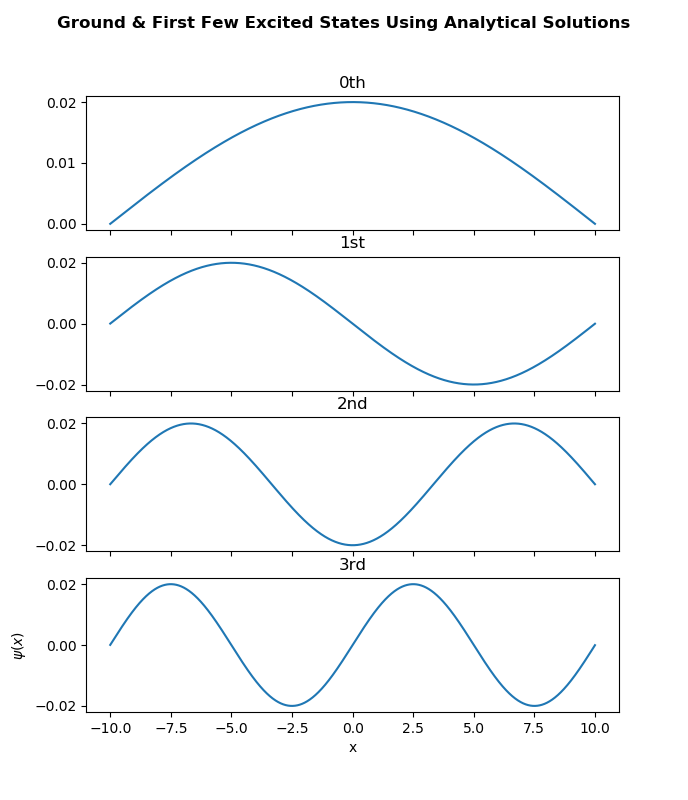
\includegraphics[width=0.5\textwidth]{./particleinabox.png}
	\centering
	\caption{Expected First Few Excited States for a Particle-In-A-Box System}
\end{figure}

\subsection{Three-Point CFD, FFD, BFD Results with no Potential (Particle In A Box)}
\begin{figure}[H]
	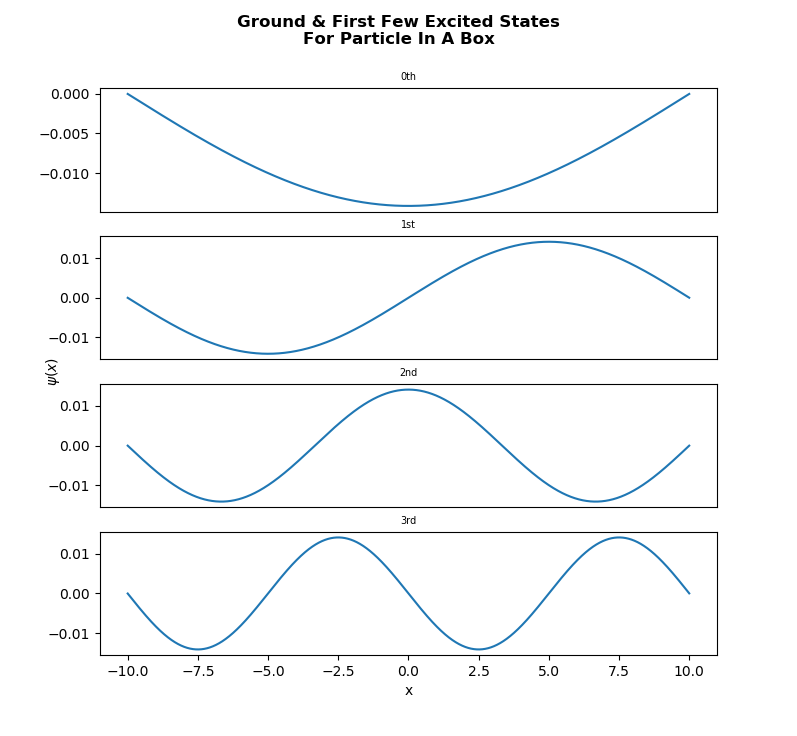
\includegraphics[width=0.75\textwidth]{./particleinaboxCFD.png}
	\centering
	\caption{First Few Excited States of Particle-In-A-Box System Calculated by CFD}
\end{figure}

These results qualitatively mimic the expected ones very closely, with the same numbers of nodes, symmetries, and constant wavelengths. This provides a good indication that this is a good method to use for other, more extravagent, models.

\begin{figure}[H]
	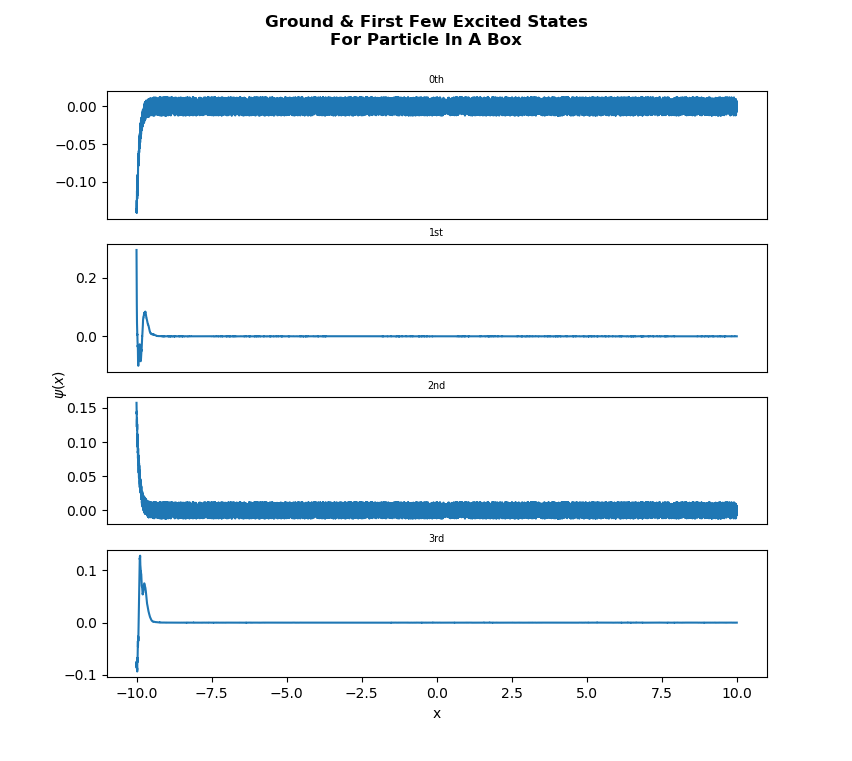
\includegraphics[width=0.75\textwidth]{./particleinaboxFFD.png}
	\centering
	\caption{First Few Excited States of Particle-In-A-Box System Calculated by FFD}
\end{figure}

\begin{figure}[H]
	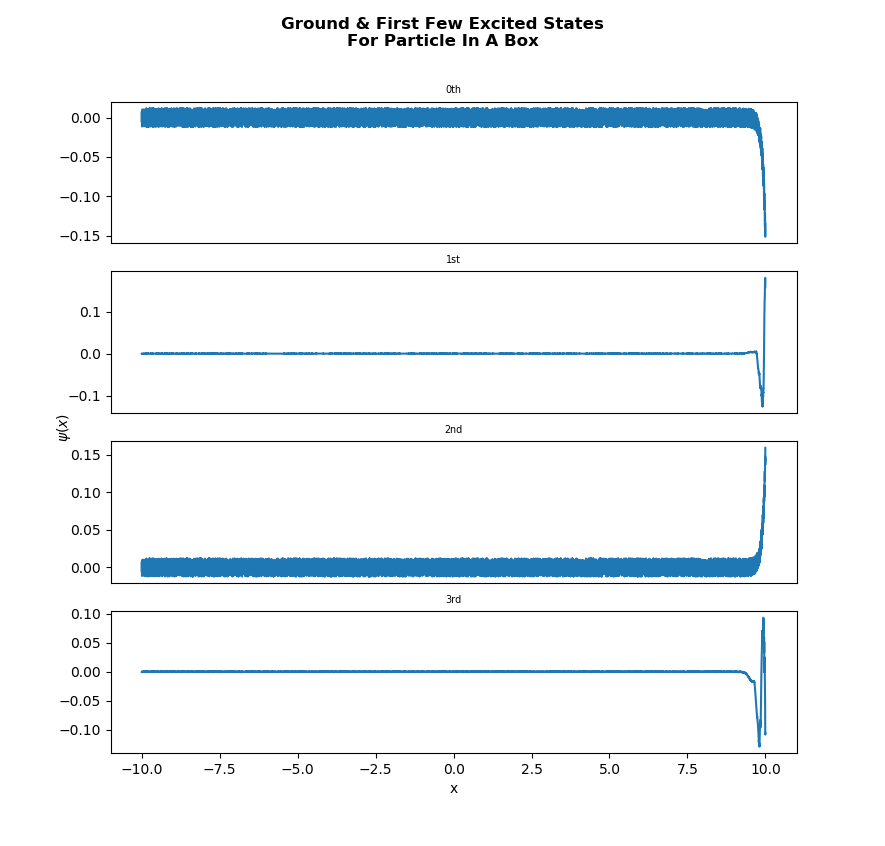
\includegraphics[width=0.75\textwidth]{./particleinaboxBFD.png}
	\centering
	\caption{First Few Excited States of Particle-In-A-Box System Calculated by BFD}
\end{figure}

For both the Forward and Backwards Finite Difference calculations, large stability issues are easily seen. As the same order of finite difference method, and so the same computational expense, was used in all three of these calculations, it is clear that the CFD method is the only one worth developing further. As stated earlier, the CFD method should be accurate to $O(h^{2})$, while the FFD and BFD methods are only accurate to $O(h)$ - this combined with decreased stability resilience resulted in the above calculations, which are not representative of the analytic solutions at all.

\section{Optimisations}

\subsection{Sparse Storage}
The first improvement to the chosen implementation (matrix method) involved moving from storing the Hamiltonian in a standard storage format, in this case a numpy ndarray, to a more suitable data structure; a sparse matrix. 

The motivation for this is that to obtain a solution to a very high accuracy a large number of grid points are needed and, with ndarray storage, the memory needed to store the Hamiltonian scales with the square of the number of grid points - meaning that the maximum possible accuracy is limited by the size of the Hamiltonian that can be held in memory. 

From <ref earlier>, we see that the Hamiltonian is tri-diagonal for our 3 point CFD approach. As a result we know everything about the Hamiltonian if we know its tri-diagonal elements, and so switching to a sparse diagonal storage data structure (scipy's sparse.diags) we can throw away the unneeded zeros and obtain a more efficient Hamiltonian representation that scales linearly with the number of grid points. 

Switching to this data structure expanded the maximum size of Hamiltonian that could be held in memory on my laptop (8GB RAM) from one using 20 thousand grid points to one using over 10 million grid points.

Limitations of this data structure include that more specialised functions are needed to operate on sparse matrices; for example numpy's linalg.eig eigensolver is unable to operate on sparse data. Luckily, scipy's sparse library has a range of equivalent tools designed to replicate the effects of many of numpy's operations for sparse data structure, including several eigensolvers which we now look at as an additional optimisation method.

\subsection{Eigensolver Choice}
As seen in the above section, a sparse storage system allows for more accurate calculations to be performed. There are two main sparse eigensolvers available to use in place of numpy's linalg.eig here; scipy's sparse.linalg.eigs and sparse.linalg.eigsh. These both work similarly, using Arnoldi-based methods for subspace iteration to obtain the eigenpairs, with the difference being that the former uses standard Arnoldi iteration, while the latter uses Lanczos iteration * CITE *. 

Lanczos iteration is a simplification of Arnoldi iteration for the case where the matrix in question is Hermitian; from * cite previous *, we know that a CFD-based Hamiltonian will be real and symmetric - and therefore Hermitian. 

Additional optimisations involving this eigensolver are possible, including the optional parameter `k' which allows the number of desired eigenstates to be specified. By default, the `k' most dominant eigenstates will be returned (dominant implying largest eigenvalue magnitude). 

As we only care about bound states, with eigenvalues below zero, we don't necessarily want the `k' most dominant eigenstates; rather we want the `k' most dominant eigenstates *corresponding to negative eigenvalues*. 

Another optional parameter, `sigma', can be used to achieve this. `sigma' allows a `target' eigenvalue value to be given and, through performing shift-invert preconditioning (* cite my L3? *), the `k' eigenstates closest to that value be returned. 

By passing in a suitably large negative number, we ensure that the returned eigenstates will correspond to the ground state and `k-1'-first excited states. This allows a massive reduction in computational effort needed to obtain particular bound states as, without these, all eigenstates would need to be calculated and then sorted. 

For a model TISE solution using a model with 10k grid points to obtain only the Ground State, and using an estimate for the ground state for the `sigma'/Shift-Invert parameter within 10\% of the real value, the eigsh routine on average took 93.421\% of the time that the eigs routine needed to converge - averaged over 7 trials. 

For the same model and goal; when an estimate that was very far off the real value (around 200 times the real value) was used instead in the Shift-Invert parameter, the eigsh and eigs routines performed very similarly to each other - with eigs being 0.5\% faster averaged over 7 trials.

Using 1 million grid points very similar results were obtained, with eigsh taking 94.753\% as long as eig with the good estimate and 99.832\% as long with a the bad estimate - based on this, it seems the benefit of using eigsh does not scale with Hamiltonian size.

Switching to calculating the Ground state and first 9 excited states, with a 10k grid point model, the benefit of eigsh over eigs for the accurate esetimate appeared to decrease slightly - taking 97.933\% as long, and again for the bad estimate they took very similar times - with eigsh taking 100.263\% as long as eigs.

Additional optimisations involving the `sigma' parameter are described below, which lead to further large reductions in computational expense.

\subsection{FastBOI Improvement}
An additional efficiency improvement that I developed makes use of results from (* cite previous *), where it is seen that the rate of convergence of an eigenstate during subspace iteration is proportional to the magnitude of the corresponding eigenvalue and that eigenstates of of a matrix are also eigenstates of that matrix's inverse (if it exists), with corresponding eigenvalues equal to the reciprocal of the original eigenvalues. 

Combining these it can be seen that if an estimate of an eigenstate's eigenvalue is known, say $\lambda$, then $\lambda I$ can be subtracted from the original matrix to create a new matrix with the same eigenstates, but with eigenvalues equal to the original ones minus $\lambda$. 

As a result, the eigenstate desired will have a `new' eigenvalue of $0$ (or very near, depending on accuracy of the estimate) - thus, if we invert the matrix, the result will have the same eigenvectors but reciprocal eigenvalues, which in the case of the desired eigenstate will be very large and tend towards $\infty$ with increasing accuracy. 

Using the knowledge that the rate of convergence is proportional to eigenvalue magnitude, this shifted and inverted matrix will converge extremely rapidly to the desired eigenstate during subspace iteration, with increased speed if the accuracy to which the original estimate is known is increased.

Based on this result, I developed a `Fast Boosted Optimiser Iteration' method to improve convergence rates for the eigensolver used to find bound states from my Hamiltonian. Another result used in the development of this approach is that a model with fewer grid points than another should still produce relatively correct eigenstates and eigenvalues, simply to a lower accuracy than a model with more grid points. 

Based on these results, the general idea of this approach is to find the ground state eigenvalue for a model with a greatly reduced number of grid points, and then use this as an estimate in the `sigma' parameter of the eigensolver for the model with full number of grid points - greatly increasing the convergence rate for the full model at the cost of having to solve an extra, much smaller, problem. 

Additionally, although only useful for models with a very large number of grid points, this approach can be stacked; a small model can generate an estimate ground state eigenvalue for a medium sized system, which can then generate a better estimate for the full very large system. A flow-chart describing the basic approach is described below, followed by adaptions to allow several `boosting' stages.

Basic FastBOI algorithm:

\begin{figure}[!htb]
	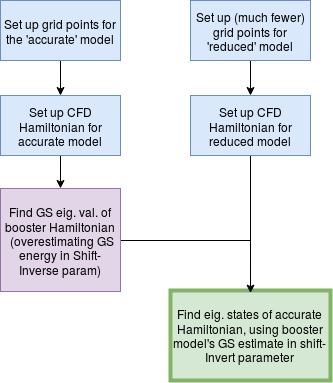
\includegraphics[scale=0.5]{FastBoi}
	\centering
	\caption{Basic FastBOI algorithm}
\end{figure}

Improved (multi-stage) FastBOI algorithm:
\begin{figure}[!htb]
	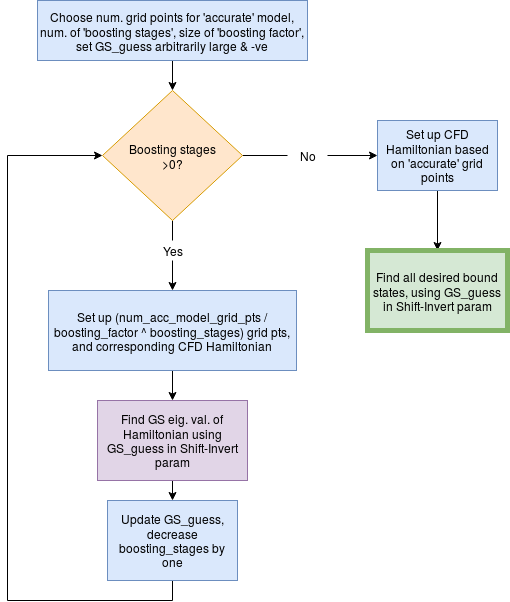
\includegraphics[scale=0.5]{FastBoiImproved}
	\centering
	\caption{Improved (recursive) FastBOI algorithm}
\end{figure}

Using a model with 50 thousand grid points, only seeking the Ground State, and using a very large negative number (around $10^{3}$x the real energy) as the baseline estimate - using the FastBOI algorithm with a boosting factor of 100 and a single boosting stage was 90.948 times faster than not using it, jumping to 107.928 times faster when the boosting factor was increased to 1000. 

Using the same comparison, but with a 500 thousand grid point model, the FastBOI algorithm with 1 boosting stage and a boosting factor of 100 was 58.914 times faster than without, with 1 boosting stage and a boosting factor of 1000 it was 77.749 times faster, and with 2 boosting stages and a boosting factor of 100 it was 87.1 times faster. 

It was noticed that the time to solve the model without using the FastBOI algorithm scaled linearly with model size - and so for the following, larger, models estimates were used for the comparisons as each calculation woud otherwise take several hours. With this assumption; for a model with 5 million grid points and only seeking the ground state, the FastBOI algorithm with 1 boosting stage and a boosting factor of 1000 was about 89 times faster, with 2 boosting stages and a boosting factor of 250 it was about 96 times faster, with 3 boosting stages and a boosting factor of 40 it was about 93 times faster, and with 4 boosting stages and a boosting factor of 10 it was about 85 times faster.

Larger models were uable to fit into RAM on my laptop, and so could not be tested.


%definition of variables:
%\begin{itemize}
%
%	\item[-]{\textbf{x_full:} The grid points for the full accuracy model}
%	\item[-]{\textbf{x_red:} The grid points for the reduced accuracy model, it will have the same start- and end-points as x_full}
%	\item[-]{\textbf{boosting_factor:} The relative size of x_full to x_red}
%
%\end{itemize}

%\begin{lstlisting}
%function basic_fastboi(x_full, boosting_factor){
%	start, end, size = x_full[0], x_full[last], SIZE(x_full);
%	inc = (end - start) / (size / boosting_factor);
%	x_red = ARRAY();
%
%	for i = 0..(size / boosting_factor){
%		x_red[i] = start + i*inc;
%	}
%
%	H_red = generate_hamiltonian(x_red); 
%	est_GS_eigval, est_GS_eigvec = eigensolver(H_red, sigma = -B);
%	
%	/* where B is some arbitrarily large number such that B
%	   is definitely less than the real GS eigenvalue.
%	   Note: matching the output of ARPACK and LAPACK eigensolver outputs,
%	   only est_GS_eigval needed
%	*/ 
%	
%	H_full = generate_hamiltonian(x_full);
%	acc_GS_eigval, acc_GS_eigvec = eigensolver(H_full, sigma = est_GS_eigval);
%	
%	return (acc_GS_eigval, acc_GS_eigvec);
%}
%\end{lstlisting}
%
%As mentioned, this `boosted optimiser' approach can be stacked iteratively allowing a more accurate estimate to be generated for the full accuracy model, at less than the cost of solving a medium size model with an arbitrarily large negative number that would otherwise be needed. The adaption to the above algorthm to allow several boosting stages is described as follows, using a recursive approach;
%
%\begin{lstlisting}
%function fastboi(x_full, boosting_factor, num_boosts, estimate=-B){
%	start, end, size = x_full[0], x_full[last], SIZE(x_full);
%	inc = (end - start) / (size / (boosting_factor^num_boosts));
%	x_red = ARRAY();
%
%	for i = 0..(size / boosting_factor){
%		x_red[i] = start + i*inc;
%	}
%
%	H_red = generate_hamiltonian(x_red); 
%	est_GS_eigval, est_GS_eigvec = eigensolver(H_red, sigma=estimate);
%	
%	if (num_boosts > 0){
%		return fastboi(x_full, boosting_factor, num_boosts-1, est_GS_eigval);
%	}
%	else{
%		H_full = generate_hamiltonian(x_full);
%		acc_GS_eigval, acc_GS_eigvec = eigensolver(H_full, sigma = est_GS_eigval);
%		return (acc_GS_eigval, acc_GS_eigvec);
%	}
%}
%\end{lstlisting}
%
\subsection{Pre-Trained Predictive Model Improvement}

An alternative to the Boosted Optimiser Iteration method, suitable for other use cases, is to find estimates to the Ground State energy for many differently shaped potentials and train a predictive model to generate an estimate to use for the Shift-Invert parameter of the eigensolver based on the shape of the potential being used. To investigate this approach I used reduced models with 1000 grid points, and generated 1000 different potentials. 

For each model I then found the ground state eigenvalue, using a massively negative estimate in the Shift-Invert parameter, and then recorded the ground state value along with statistics to describe the potential used in that model; such as mean, median, skew, standard deviation, kurtosis. 

Several machine learning models, including a 3-hidden-layer neural network and a boosted random forest, were trained on a randomly selected 85\% of the data. After feature selection and hyperparameter tuning, the models ranged from 97.3\% (simple linear regression) to 99.996\% (neural network) accurate on the unseen 15\% of the data (measured using Mean Average Error).
Once trained, these predictive models can be saved for future usage - allowing for a near-immediate Ground State estimate in the future as opposed to having to solve one or more reduced models every time. 

Using a prediction from the neural network model in the Shift-Invert parameter when solving a 10k grid point model gave around a 400x speedup compared to using a large negative guess - including the time taken to generate statistics about the potential and feed them into the neural network. 

Limitations of this approach include that, unless similar calculations are going to be performed often, the time taken to generate the synthetic data and train the predictive model is much greater than the cost of not using a good ground state estimate, and also that this approach can't `stack' like the Boosted Optimiser Iteration approach - limiting the speedup benefit for very high-precision models. 

Advantages of it are that, once trained, there is very little extra work or computational effort needed to allow the speedup, and also over time the higher-accuracy ground state energies that are calculated can be saved and the predictive model retrained using them.


%----------------------------------------------------------------------------------------
 
% Chapter 1

\chapter{TDSE Solution \& Optimisation} % Main chapter title

\label{Chapter3} % For referencing the chapter elsewhere, use \ref{Chapter1} 

%----------------------------------------------------------------------------------------


\section{Time Evolution of a Quantum State}
\subsection{Exact Solutions and Limitations}
The evolution of a quantum state can be described fully by the Schr$\ddot{o}$dinger equation, in it's time-dependent form, which we will refer to from now as the TDSE. The TDSE states that an arbitrary quantum state, $\Psi$, will evolve according to;
$$ 
i \hbar \frac{\partial}{\partial t} \Psi=H \Psi,
$$
where H is the Hamiltonian of the system, and is in general also time-dependent. We now consider the case where the Hamiltonian does not evolve with time - this is a much easier case to solve, in fact only a few particular systems with non-constant Hamiltonians are analytically solvable. We will investigate these numerically later in this chapter.

Solving this equation, we obtain 
$$
\Psi\left(t\right) = e^{\frac{i}{\hbar}Ht}\Psi\left(0\right),
$$
where a constant of integration has been neglected as it amounts to a global phase-shift.

By spectrally decomposing $\Psi$ into it's component eigenstates, $\sum_{i}{c_{i}\mathbf{e_{i}}}$, we can rewrite this as;
$$
\Psi\left(t\right) = \sum_{j}{e^{\frac{i}{\hbar}\lambda_{j}t}c_{j}\mathbf{e_{j}}\left(0\right)},
$$
allowing us to see that each individual eigenstate oscillates in amplitude, with a frequency determined by the energy of the eigenstate.

Solutions for this case can therefore be exactly calculated if the eigenstates are known, and so we can use this case to compare to our numerical model solutions to measure their accuracy.

\subsection{The Case for Numerical Methods}
The TDSE is not trivially solvable analytically other than for particular time-dependent Hamiltonians; and so to be able to investigate the time evolution of more complicated systems, or systems with more complicated external potentials, a different approach must be used. 

One alternative approach is pertubation theory, where known solutions to Hamiltonians of simpler systems are used to approximate the more complicated systems along with small additional `perturbative' terms. This approach's accuracy is mostly limited by the size of the pertubation, and so is useful for modelling the evolution for systems similar to an analytically solvable one with a small additional term - but not in the general case for modelling arbitrary systems.

Another approach is to use numerical methods; discretizing the Hamiltonian and wavefunction and using numerical solutions to the differential equation by approximating derivatives with series or basis expansions - as we did for the numerical solutions to the TISE. 

Advantages of this approach include that computers are easily able to compute solutions to discretized models, and that these approaches are not limited to systems similar to analytically solvable ones - as they do not rely on the solutions to the differential equation being similar, instead solving the differential equation in a completely different way.

In this chapter we investigate and compare two numerical methods of solving the TDSE; a Finite Difference propagator, and a Krylov Subspace propagator. These both work similarly, using one or more previous states of the wavefunction to predict the state at the next timestep, and updating the Hamiltonian at ever timestep.

\section{Finite Difference Propagator}
A finite difference approach to this problem is very similar to the one used in solving the TISE - with the main difference being that we are now propagating in time rather than space. Additionally, as we don't know anything about the wavefunction at points in time ahead of the current timestep, we can't use any backwards terms in our finite difference scheme. 

FD methods require knowledge of the wavefunction at several initial timesteps to be able to start to propagate; in the TISE solution we took the initial points to be all $0$, but that is an unsuitable assumption for this case. 

Instead, we use analytic solutions to the field-free case to build up the first few timesteps. This is equivalent to assuming that no external potential is applied to the system for the first few timesteps, which is a much more realistic assumption.

\section{Krylov Subspace Propagator}
The Krylov Subspace approach works differently, calculating the state of the wavefunction at the next timestep in terms of only the current one. 

To do this, a krylov subspace is built from a matrix representation of the Hamiltonian at the next timestep and using the current wavefunction as the starting vector for the subspace. 

The vectors in the subspace are then added, weighted by appropriate taylor series coefficients, to give the approximation for the wavefunction at the next timestep. This approximation increases in accuracy with increased subspace size, although almost all information is contained in the first few terms and there is a rapidly decreasing benefit to additional subspace elements - the rate of the descrease here is considerably greater than the decrease in benefit of using additional finite difference terms in the FD propagator case. However, the computational costs of using more terms are not the same in both propagators and so it is non-trivial to determine which method is more efficient in any given case - this will be discussed later in this chapter.

To summarise the process;
First the Krylov subspace, $\mathbb{K}$, is built:
$$
\mathbb{K} = \left[\Psi\left(t\right) ,\ H\left(t+\delta{t}\right)\Psi\left(t\right) ,\ H^{2}\left(t+\delta{t}\right)\Psi\left(t\right) ,\ ... \right]
$$
Then a weighted sum of the subspace elements, $\{k_{i}\}$, is used to approximate $\Psi\left(t+\delta{t}\right)$:
$$
\Psi\left(t+\delta{t}\right) = \sum_{i}{\frac{-i\delta{t}^{i}}{i!}k_{i}}
$$

Advantages of this approach include accurate convergence with relatively few terms needed, and that there is no need for the first few terms to be analytic solutions to the field-free case.
Disadvantages of it include that a large matrix-vector multiplication must be performed for every term in the approximation, as opposed to a single one regardless of the number of terms in the FD approach.
%This 'baseline solution' finds the first $k$ eigenstates of the Hamiltonian associated with an elecron interacting with a Hydrogenic atom at an instant, with the Coulomb Potential being modelled instead by a Soft-Core potential - which at all but very small distances is an accurate approximation of the Coulomb Potential. Due to the Coulomb Potential tending towards $\infty$ as $r\rightarrow 0$ it is difficult to model it numerically, but with a Soft-Core Potential approximation, we avoid the issues at small $r$s yet obtain accurate results for everywhere other than at the center.

\section{Comparisons Between Time Propagators}

\subsection{Efficiency Comparisons For 6000 Timesteps With A Small Grid}
Using only the constant Soft-Core potential, and so with no time-dependent terms in the Hamiltonian, the two propagators were used to propagate the Ground State wavefunction 6000 timesteps - using a 1000 grid points to represent the wavefunction, a timestep of $10^{-3}$ atomic units of time, and both propagators using 6 terms. The results shown are averaged over 5 repeated calculations. 

For context if attempting to reprodce the results, the calculations were performed in a Python3.7 Jupyter Notebook, running on a 3.2GHz i7u processor with 8GB of RAM.

\subsubsection{Krylov Subspace Propagator:}
Mean runtime: \hspace{2cm} 32.28598s\newline
Standard Deviation: 0.10144s / 0.31419\%

\subsubsection{Finite Difference Propagator:}
Mean runtime: 26.62208s\newline
Standard Deviation: 1.18747s / 4.46047\%

\textbf{Note:} It was noticed for this set of results that 4 runs were extremely close to 26s, with a single result being almost 29s. The cause of this anomaly was investigated and was determined to be that I switched to a different browser tab during that calculation; Facebook, which loads a number of videos and images when opened. The anomalous result was replaced with 3 new calculations to instead give the following results;\newline
Mean runtime: \hspace{2cm} 26.02711s\newline
Standard Deviation: 0.10275s / 0.39478\%

Additionally, I attempted to recreate the anomalous result by averaging 5 calculations during which I switched to the Facebook tab, in order to support the hypothesis that the extra compuatational power required by facebook caused the anomalous result. The results of that attempt were as follows;\newline
Mean runtime: \hspace{2cm} 33.73616s\newline
Standard Deviation: 5.19175s / 15.38927\%

\subsubsection{Analysis:}
From these results, it is clear that for this setup the Finite Difference propagator performs more efficiently - taking only around 80\% of the time as the Krylov Subspace propagator. Additionally, both propagators had a very similar spread of times taken; showing that each is roughly as reliable as the other.

\subsection{Efficiency Comparisons For 6000 Timesteps With A Large Grid}
The previous experiment was repeated, changing only the number of grid points used to 100,000. Due to the length of time required for these calculations, they were not averaged to obtain a more accurate result and determine the spread of results; instead the spread after 500 timesteps was investigated, using 5 calculations for each propagator, afterwards to provide some insight to the expected spread of results for the full 6000 timesteps.

\subsubsection{Krylov Subspace Propagator:}
Mean runtime: \hspace{2cm} 2392.27s

\subsubsection{Finite Difference Propagator:}
Mean runtime: 2093.00s

\subsubsection{Standard Deviations after 500 timesteps:}
Krylov Subspace propagator:\newline
Mean runtime: \hspace{2cm} 198.092076s\newline
Standard Deviation: 0.62765s / 0.31685\%\newline\newline
Finite Difference propagator:\newline
Mean runtime: \hspace{2cm} 172.43040s\newline
Standard Deviation: 0.58337s / 0.33832\%

\subsubsection{Analysis:}
From the standard deviations at 500 timesteps, we can expect that at the full 6000 timesteps the standard deviations for each propagator will be very small compared to the mean - and similar in magnitude, with the Finite Difference propagator possibly having a slightly larger relative standard deviation. From this, we can conclude that for a model with many grid points the Finite Difference model outperforms the Krylov Subspace model, although to less of an extent than it does with a smaller model; taking around 87\% of the time rather than 80\%.

\subsection{Efficiency Comparisons For 60,000 Timesteps With A Small Grid}
The initial experiment was repeated, using 60,000 timesteps instead of 6,000, to investigate how the model performances scale with propagation distance. 

\subsubsection{Krylov Subspace Propagator:}

Mean runtime: \hspace{2cm} 327.40101s\newline
Standard Deviation: 0.53118s / 0.16224\%

\subsubsection{Finite Difference Propagator:}

Mean runtime: \hspace{2cm} 263.82221s\newline
Standard Deviation: 0.61104s / 0.23161\%

\subsubsection{Analysis:}
Here we see that the Finite Difference propagator still only takes about 80\% of the time to run as the Krylov Subspace propagator, matching the results for the smaller number of timesteps with the same grid size. It can also be seen that the relative standard deviations of the times taken have reduced to around half of their values for the model with fewer timesteps; this would imply that the main inconsistencies were in the setup of the models, and once that is complete there is a lower level of difference.

\subsection{Accuracy Comparisons For 6000 Timesteps Over A Small Grid}
To compare the accuracies achievable with the two methods, we are limited to cases that can be exactly solved; for this purpose we compare results for modelling field-free propagation. 

The setup of the computational experiment is mostly the same as described for the first `efficiency' test, with one difference being that the timestep size of $10^{-3}$ was found to be too large for the Krylov Subspace propagator to handle, causing massive instabilities regardless of the order of the propagator. Instead, a timestep size of $10^{-4}$ was used. 

It is worth noting that the Finite Difference propagator was able to produce reliable results even for these larger timesteps and so could be more useful in some contexts than the Krylov Subspace propagator due to this. Additionally, the fact that the end results for the Krylov Subspace propagator are completely unphysical does not detract from the findings in the above efficiencies comparison; as the number of operations performed at each timestep does not depend on the magnitude of the timestep in any way, and the number of timesteps used was kept constant.

Initially sixth-order propagators were used for each method and the accuracy is measured by comparing the population of the Ground State, i.e. the Ground State coefficient of the spectral decomposition of the propagated wavefunction, at the end of the propagation. 

Given that we use the ground state as our wavefunction, and there is no external field to excite the system, the population of the ground state should remain 1 throughout the propagation - the magnitudes of any increases or reductions to this would indicate numerical errors.

\subsubsection{CASE 1 - dt = $10^{-4}$, Grid Size = 1000, End Time = 0.6, propagation order = 6}
Krylov Subspace Error: 1.1102230246251565e-16\newline
Finite Difference Error: 2.220446049250313e-16  

\subsubsection{CASE 2 - dt = $10^{-4}$, Grid Size = 1000, End Time = 6, propagation order = 6}
Krylov Subspace Error: 0.0\newline
Finite Difference Error: -2.220446049250313e-16 

\subsubsection{Analysis:}
From these, it is clear that both are very accurate models. For clarification on the repeated result for the Finite Difference propagator, and for the fact that the first Krylov Subspace propagator result is exactly half that of the Finite Difference ones, the wavefunction is stored internally as an array of double precision floating point numbers - which have a maximum precision of -2.220446049250313e-16. Therefore the accuracy of the results are seemingly limited more by their storage medium than the fact that they are only approximations of the solution. 

Because of this, in order to determine which method is more accurate compared to the other, we must either reduce the number of terms used by each propagator or greatly increase the `end time' of the propagation.

\subsubsection{CASE 3 - dt = $10^{-4}$, Grid Size = 1000, End Time = 0.6, propagation order = 3}
Krylov Subspace Error: 3.775724177756956e-10\newline
Finite Difference Error: 0.0

\subsubsection{CASE 4 - dt = $10^{-4}$, Grid Size = 1000, End Time = 6, propagation order = 3}
Krylov Subspace Error: 3.775721957310907e-10\newline
Finite Difference Error: 1.1102230246251565e-16 

\subsubsection{Analysis:}
These results show that even when using half the number of terms in the propagators the FD method can retain accuracy to within the maximum possible tolerance of the storage medium - this was unexpected as it was believed that while the first few terms in a Krylov subspace should contain almost all of the information about the wavefunction at the next timestep, the same was not expected to be true of the FD method. One reason the FD method could be more accurate at a lower propagation order in this case is that we are investigating the ground state which is relatively smooth over the entire interval. 

Additionally, while less accurate than the FD propagator, the Krylov Subspace approach was still very accurate - and retained the accuracy when moving from the 6,000 timesteps case to the 60,000 case. This shows that the model is stable, i.e. does not contain terms that cause it to reduce in accuracy over time.

The FD propagator was further tested to failure, in order to determine how large of a timestep it could handle and still remain accurate. It was found that, with 3rd order propagation, after 6,000 timesteps it was still accurate to around machine precision for a timestep of $5e^{-3}$, for $6e^{-3}$ it had an error of 6.54306e-07, and for $7e^{-3}$ it had an error of $1$. This shows that, while it is extremely accurate and stable for small timesteps, it rapidly loses stability if the timestep is even slightly too large.

Additionally this shows that in order to approximate the wavefunction at a given time to a given tolerance, the FD approach can use both a smaller number of terms and a larger timestep - this results in orders of magnitude fewer calculations needing to be performed, allowing it to be calculated much more quickly.


For both of these propagators the critical magnitude of the timestep before instability depends on the size of the gap between grid points. We investigated this by repeating the experiments using a larger number of grid points over the same interval (100,000 vs. 1,000). As it has already been shown that either instabilities will cause the error to quickly grow, or the error will remain fairly constant during propagation if the model is stable, we only need to compare the errors after a relatively small number of timesteps in order to determine the accuracy of the model. For this purpose, we will propagate for only 300 timesteps.

\subsubsection{CASE 5 - dt = $10^{-4}$, Grid Size = 100000, End Time = 0.03, propagation order = 6}
Krylov Subspace Error: -103435.8494626187\newline
Finite Difference Error: 0.9999999999723448 

\subsubsection{CASE 6 - dt = $10^{-5}$, Grid Size = 100000, End Time = 0.003, propagation order = 6}
Krylov Subspace Error: 0.8971347740628693\newline
Finite Difference Error: 4.440892098500626e-16

\subsubsection{CASE 7 - dt = $10^{-7}$, Grid Size = 100000, End Time = 0.00003, propagation order = 6}
Krylov Subspace Error: 0.9999999999999252\newline

\subsubsection{CASE 8 - dt = $10^{-8}$, Grid Size = 100000, End Time = 0.000003, propagation order = 6}
Krylov Subspace Error: 4.440892098500626e-16\newline

\subsubsection{Analysis:}
Here we can see that when we use more grid points we need to decrease the size of the timestep to maintain stability. We see that for a grid 100 times the size, we need to decrease the the size of the timestep by around 2 orders of magnitude for the FD propagator to achieve stability, while the Krylov Subspace propagator needs the timestep to be decreased by around 4 orders of magnitude. From this we can conclude that the accuracy and stability of the solutions scale more effectively with the FD propagator than the Krylov Subspace propagator as the number of grid points increases.

%----------------------------------------------------------------------------------------


% Chapter 1

\chapter{TDSE Solutions for Time-Dependent Potentials} % Main chapter title

\label{Chapter4} % For referencing the chapter elsewhere, use \ref{Chapter1} 

%----------------------------------------------------------------------------------------
\section{Qualitative Expectation for Results}
Previously we saw that solutions to the TISE can be expressed as weighted sums of bound eigenstates, where each bound eigenstate corresponds to a distinct energy. It was also shown that if no external potential acts on the system these weights will not change as the wavefunction evolves with time; we used this fact to measure the accuracy of our propagators in the previous chapter. 

The fact that these weights remain constant with no external potential being applied is equivalent to saying that the energy of the system remains constant under time evolution; this makes physical sense as a statement of the conservation of energy. When an external field is applied, the system will either gain or lose energy over time - and so these weights will change during time evolution. 

As the weight / coefficient of each eigenstate corresponds to the probability of the system being in that state, by constructing appropriate time-dependent external potentials we can model how the probabilities of the system being in particular eigenstates changes in the event of some physical interactions; for example absorbing a laser pulse. 

The rest of this chapter consists of investigating how the system, initially in the Ground State, evolves under the influence of different simulated interactions - by investigating the change to the Ground State population under the interactions over time.

\section{Linearly Increasing Potential Field}
Here we investigate the evolution of the system under a linearly growing (w.r.t. time) potential field.

\subsection{Potential Description}
We simulate the external potential term as $\alpha t \mathbf{r}$; where $\mathbf{r}$ is the spatial interval, $t$ is the time, and $\alpha$ is a constant to determine the rate of increase of intensity of the potential.

This extra potential term was then added to the softcore potential, and the resulting total potential used along the central diagonal of the Hamiltonian.

\subsection{Effect On State Evolution}
Figure 4.1, below, shows the effect of the linearly increasing potential on the wavefunction (initially Ground State) over time.
\begin{figure}[H]
          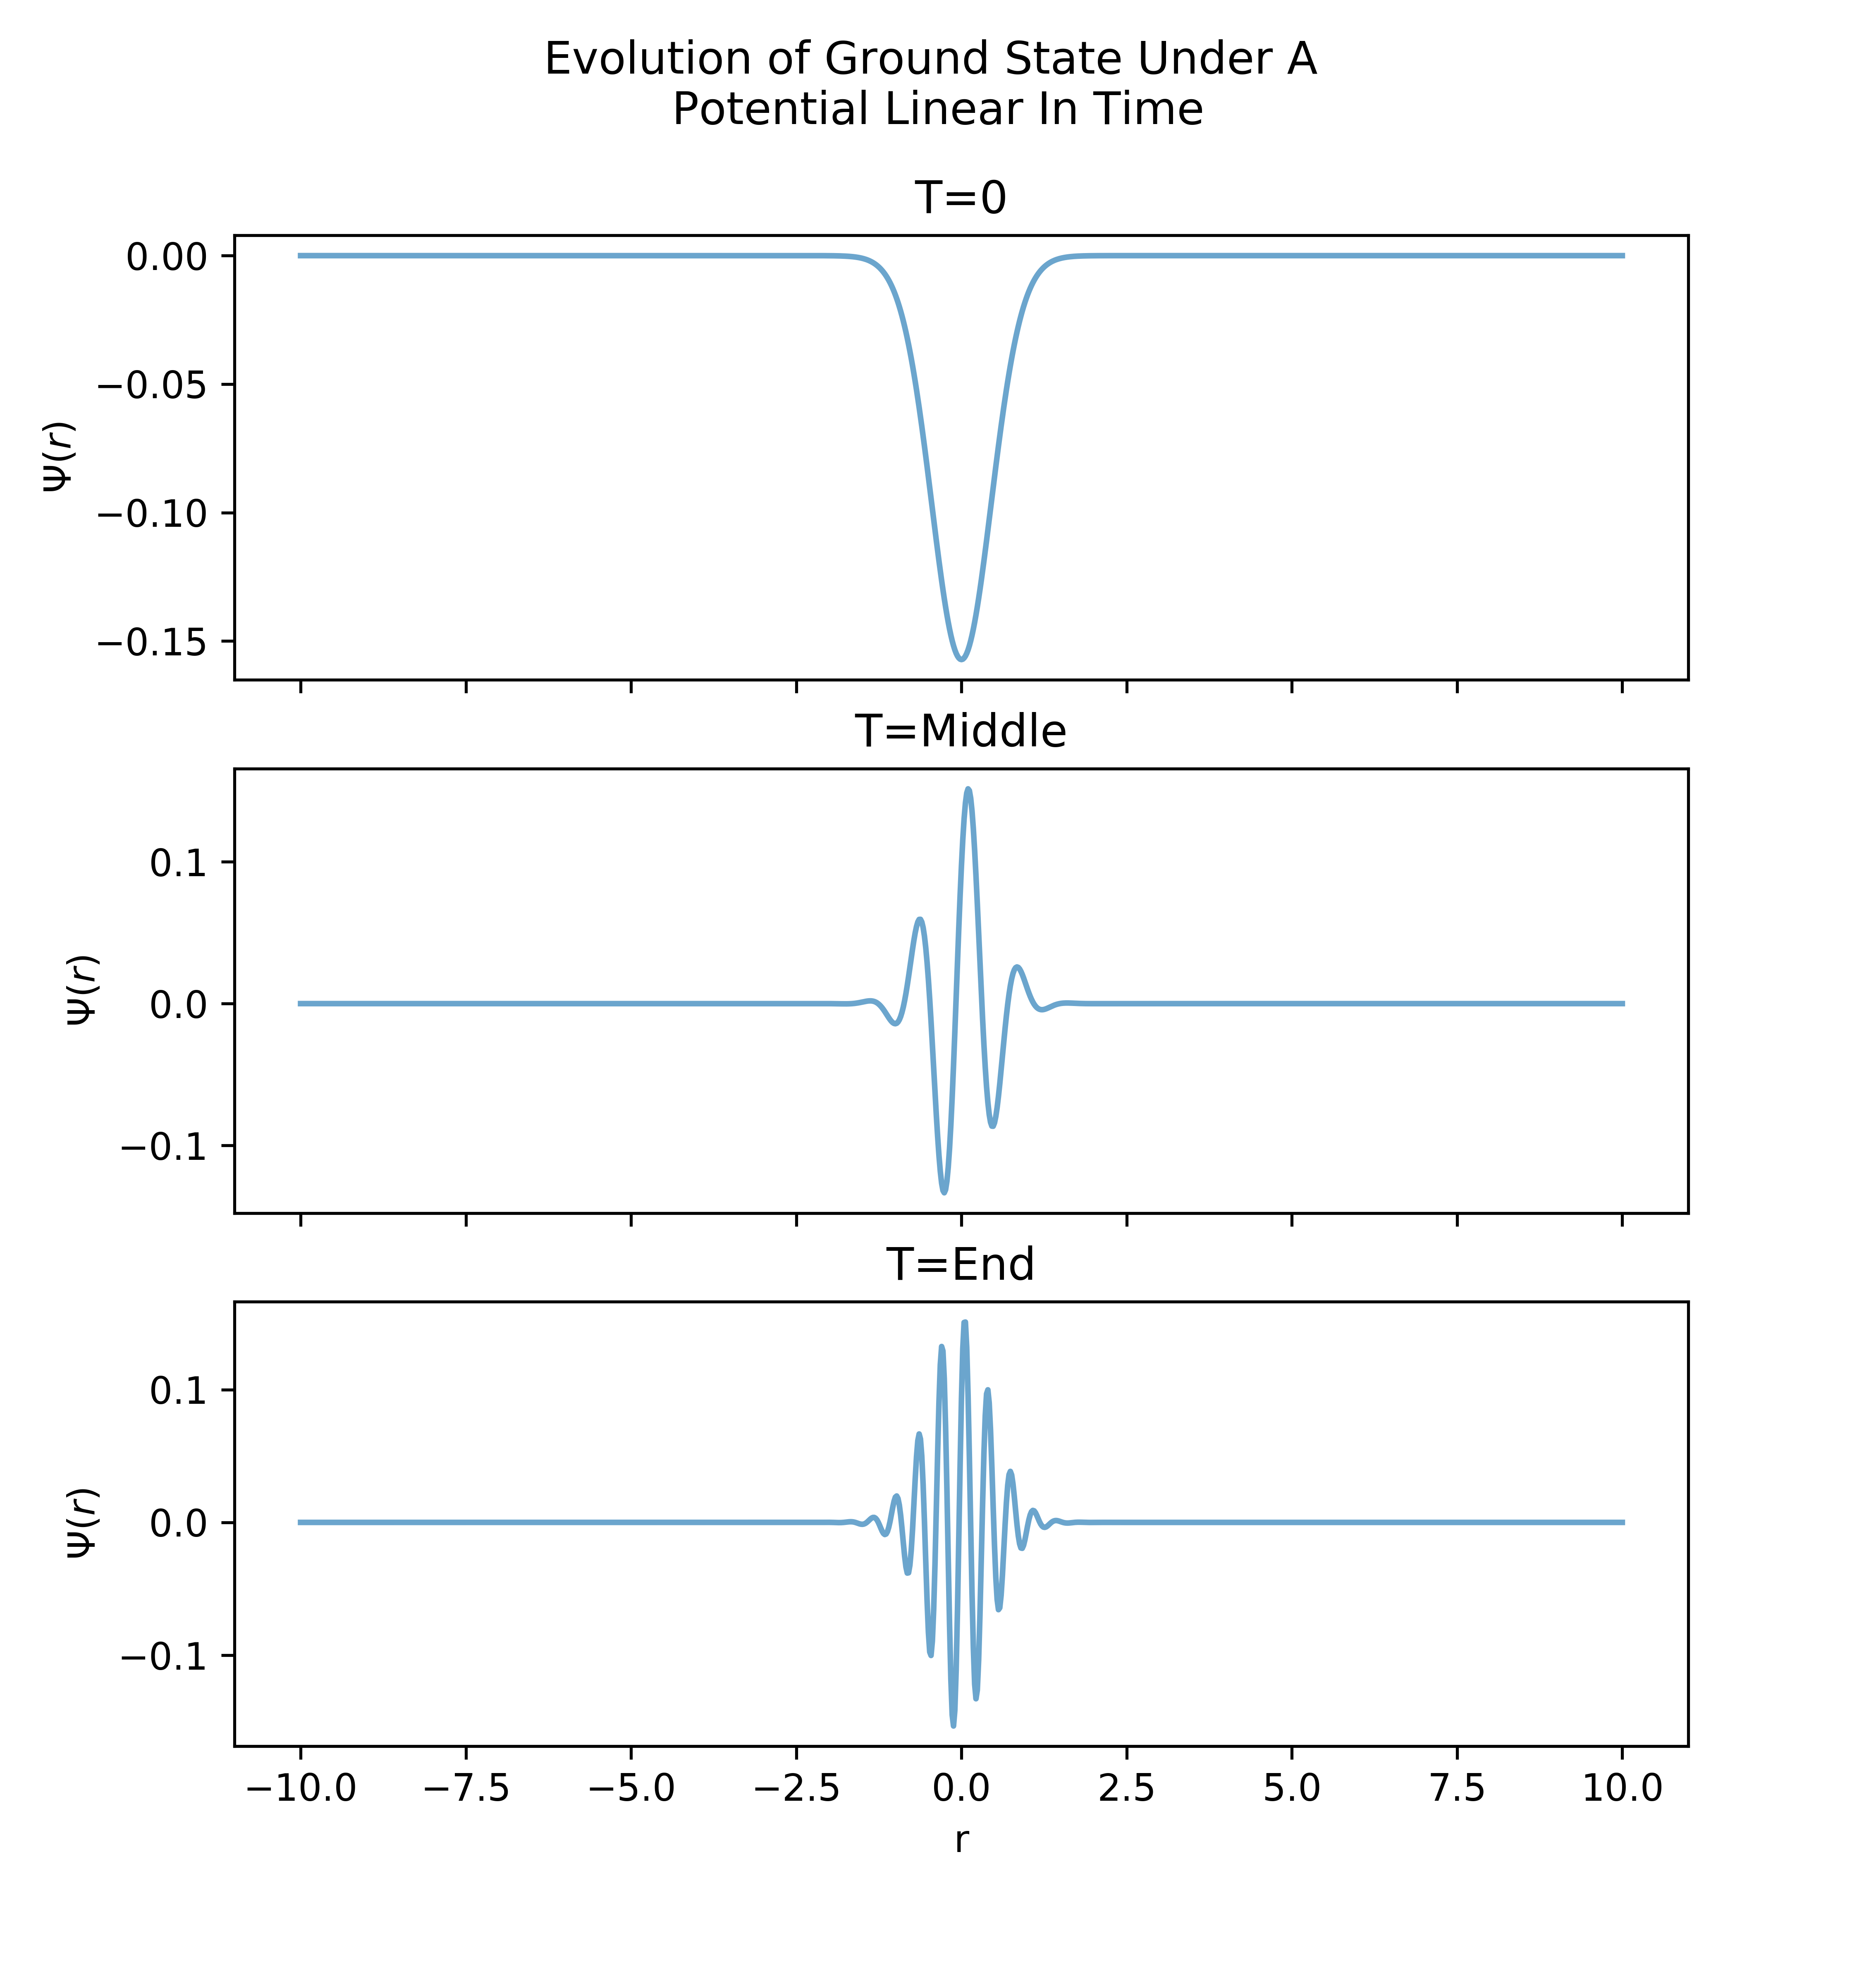
\includegraphics[width=\textwidth]{./GSLinTimeNEWwavefunction.png}
          \centering
          \caption{Effect of a linearly growing potential on wavefunction}
\end{figure}
From this figure, we see qualitatively that as time goes on the system is excited to higher and higher energies; shown through the increased numbers of turning points, and their relative magnitudes, indicating increasing contributions from higher energy eigenstates. Based on this, we can expect that the Ground State population will reduce over time as more and more eigenstates contribute and their contributions gain more and more weight. Figure 4.2, below, shows the decrease in the Ground State population over the same time interval:

\begin{figure}[H]
          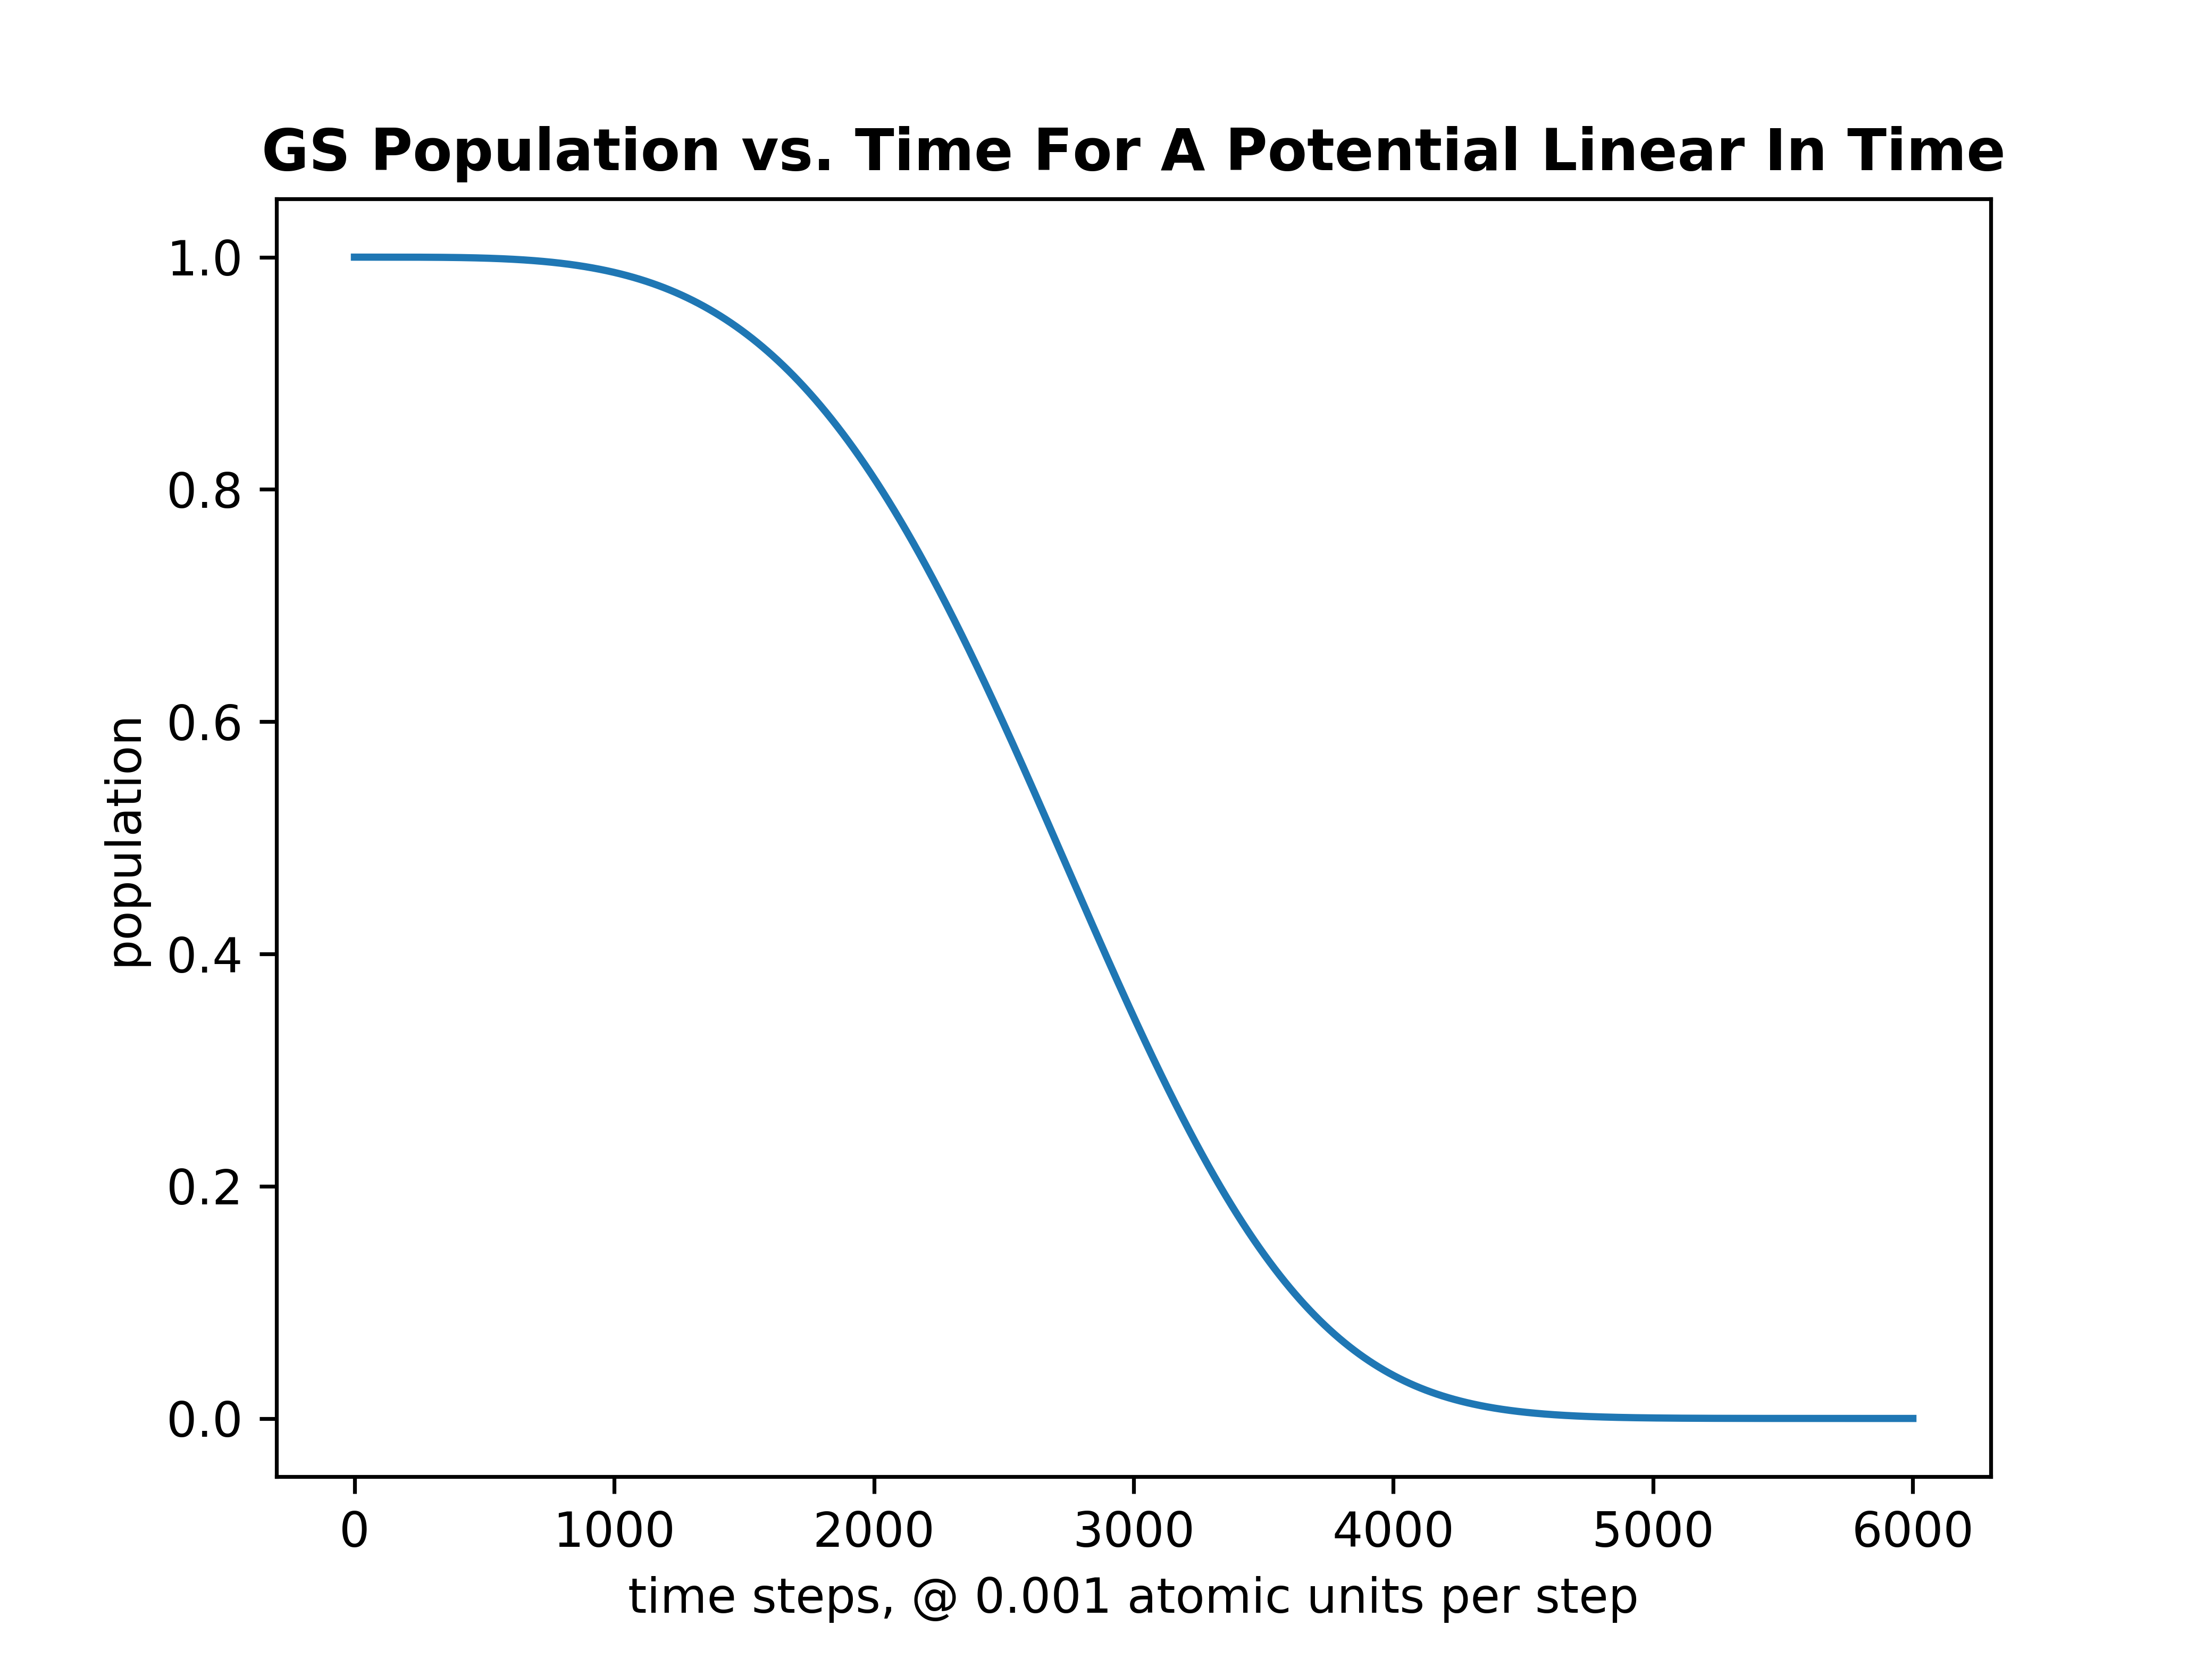
\includegraphics[width=\textwidth]{./GSLinTimeNEW.png}
          \centering
          \caption{Effect of a linearly growing potential on Ground State Population}
\end{figure}

\section{Gaussian Packet Potential}
In this section we investigate how our system would behave under the influence of a gaussian (with time) potential.

\subsection{Potential Description}
In this case, we build the external potential term as a gaussian packet w.r.t. time such that the centre of the packet (most intense part) occurs at 1 atomic unit of time, and the standard deviation of the packet is 0.25 atomic units of time. The intensity of the potential is controlled by a multiplicative factor, $\alpha$, giving the following expression for the external potential: 
$$
V_{\text{ext}} = \alpha \frac{4}{\sqrt{2\pi}}e^{-8\left(t-1\right)^{2}}\mathbf{r}
$$

As with the previous example, this extra potential term was added to the softcore potential, and the result used along the central diagonal of the Hamiltonian.

\subsection{Effect On State Evolution}

\begin{figure}[H]
          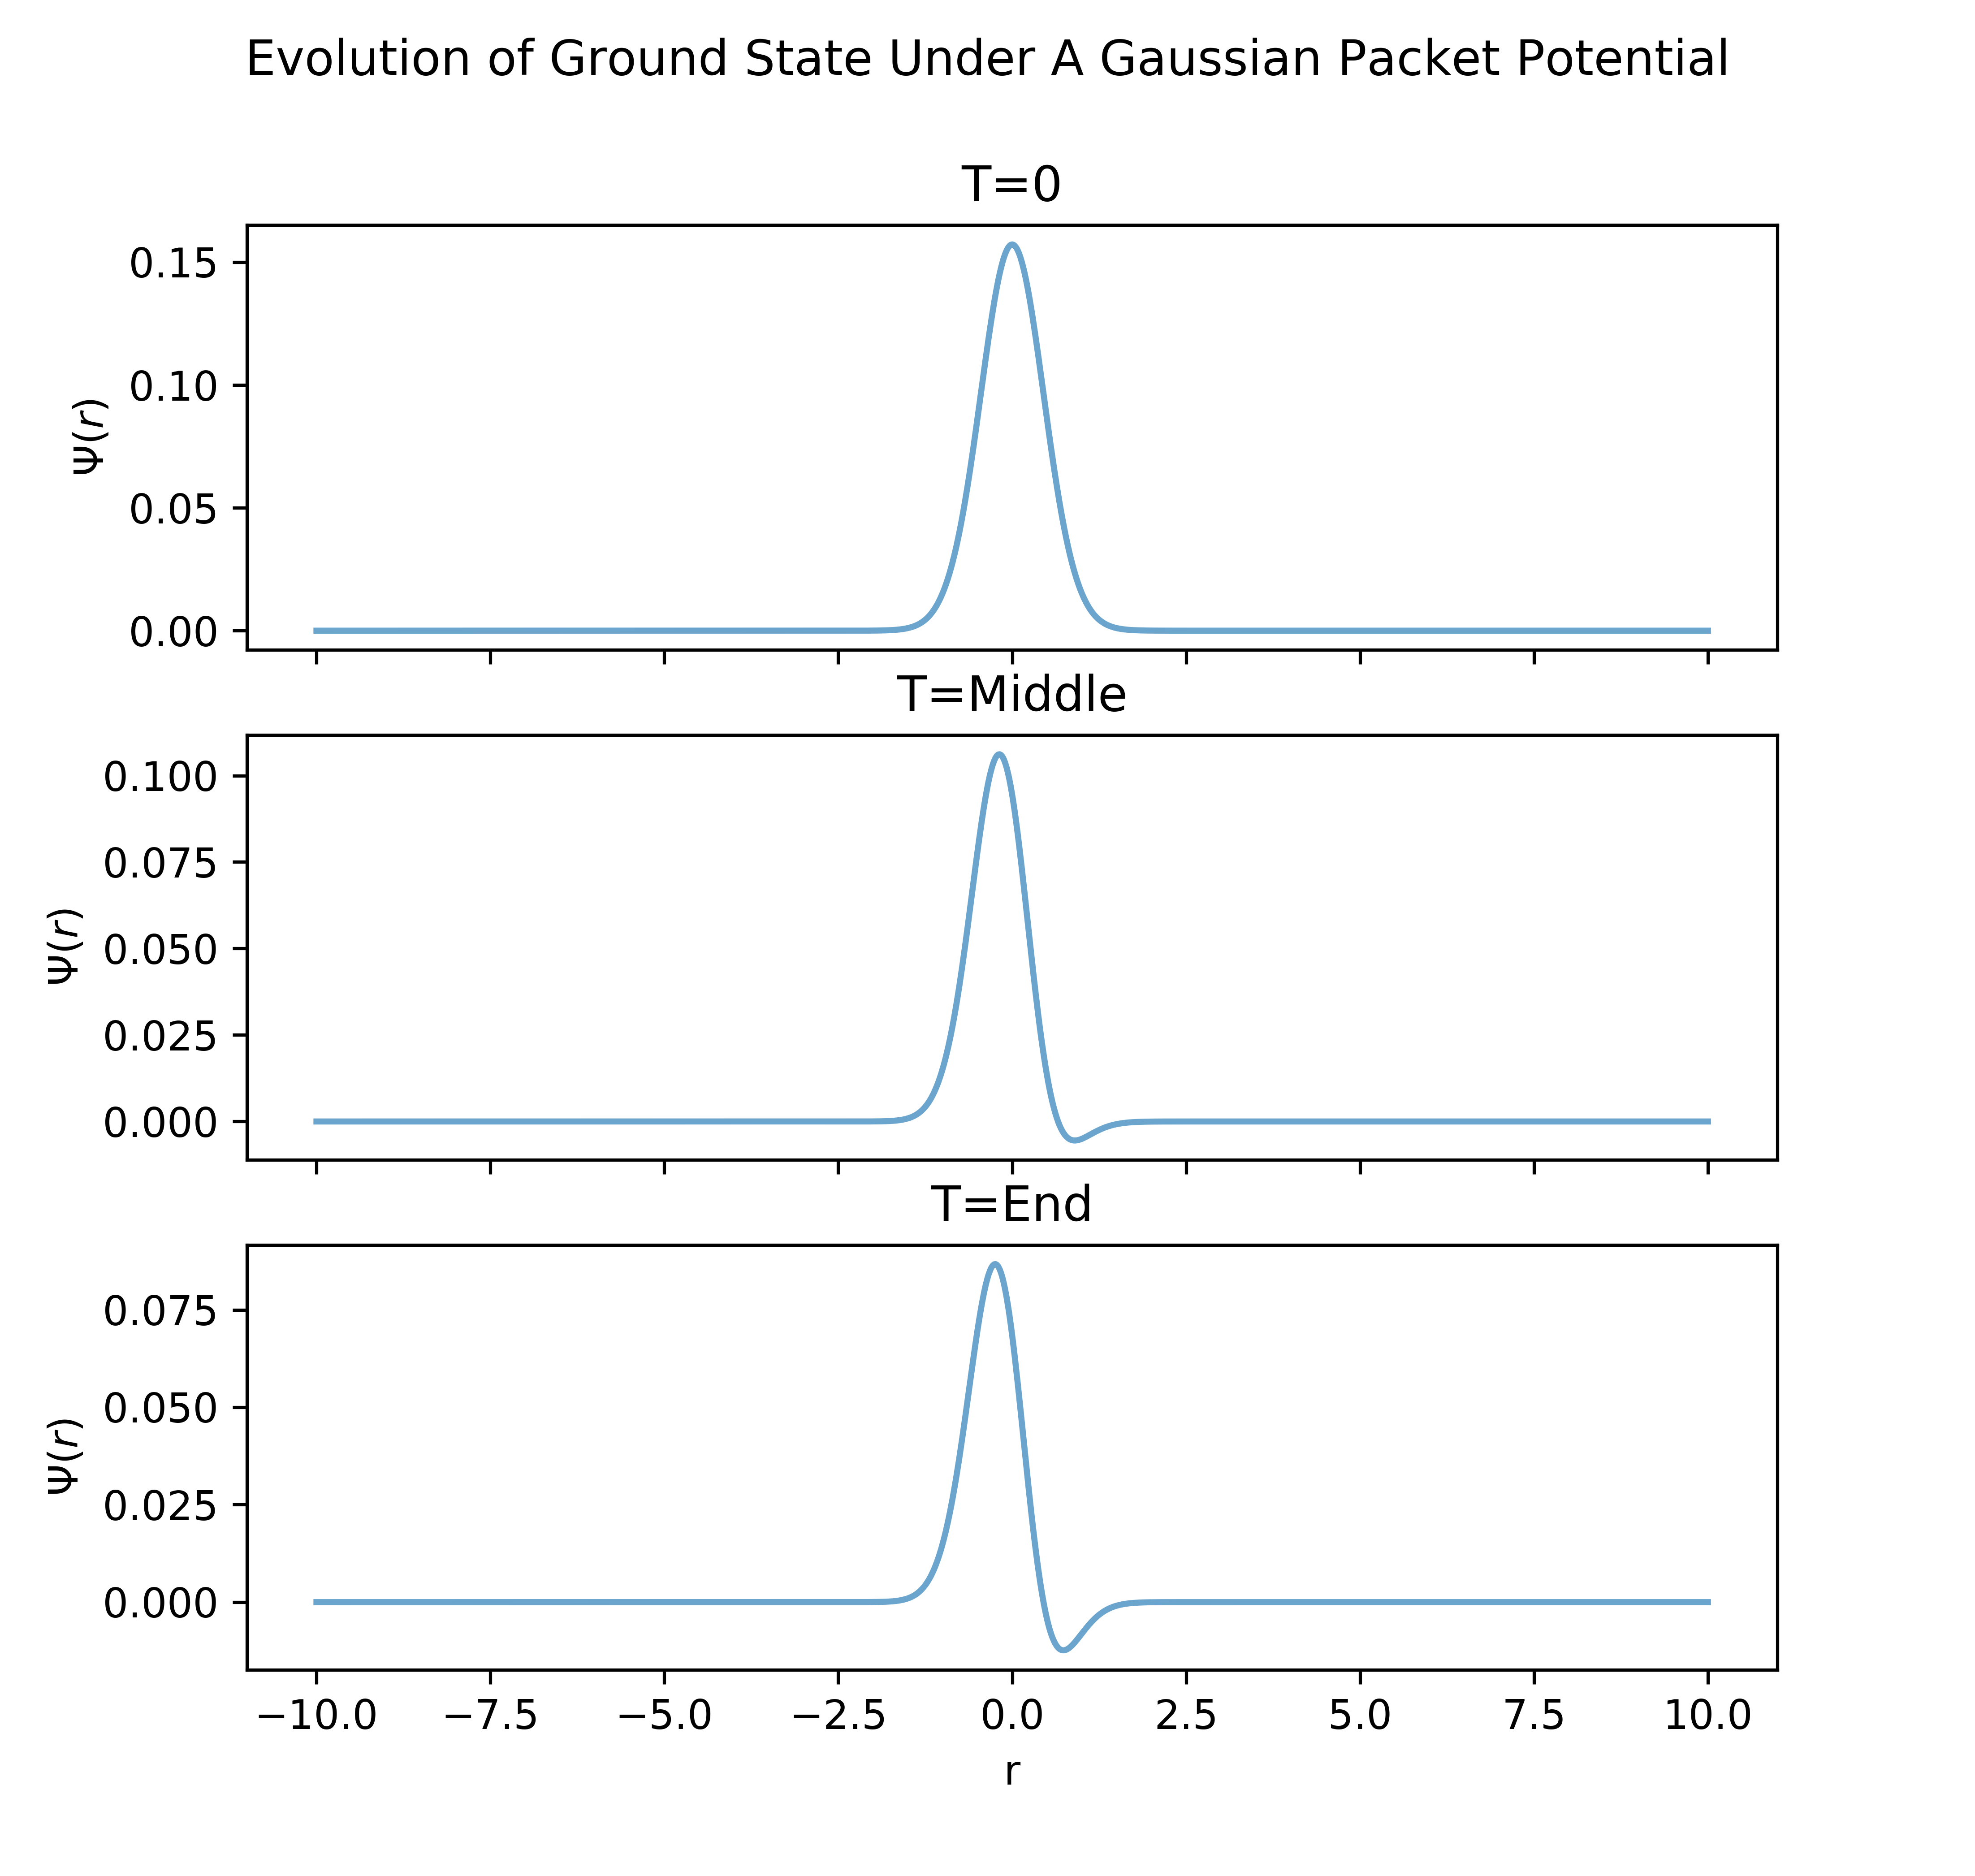
\includegraphics[width=\textwidth]{./GS1GaussianPacketNEWwavefunction.png}
          \centering
          \caption{Effect of Single Gaussian Packet on wavefunction}
\end{figure}

Figure 4.3, above, we see that almost all of a relatively small amount of energy is absorbed some time between the start and mid-point of the simulation (an interval of 3 atomic units of time), seen through the small additional turning point indicating a small contribution from the first excited state. There is very little change in shape between the mid-point and end of the simulation, indicating that there was very little incoming / outgoing energy in this time period.

The change to Ground State population was investigated over the same time interval, and the results shown in Figure 4.4, below:
\begin{figure}[H]
          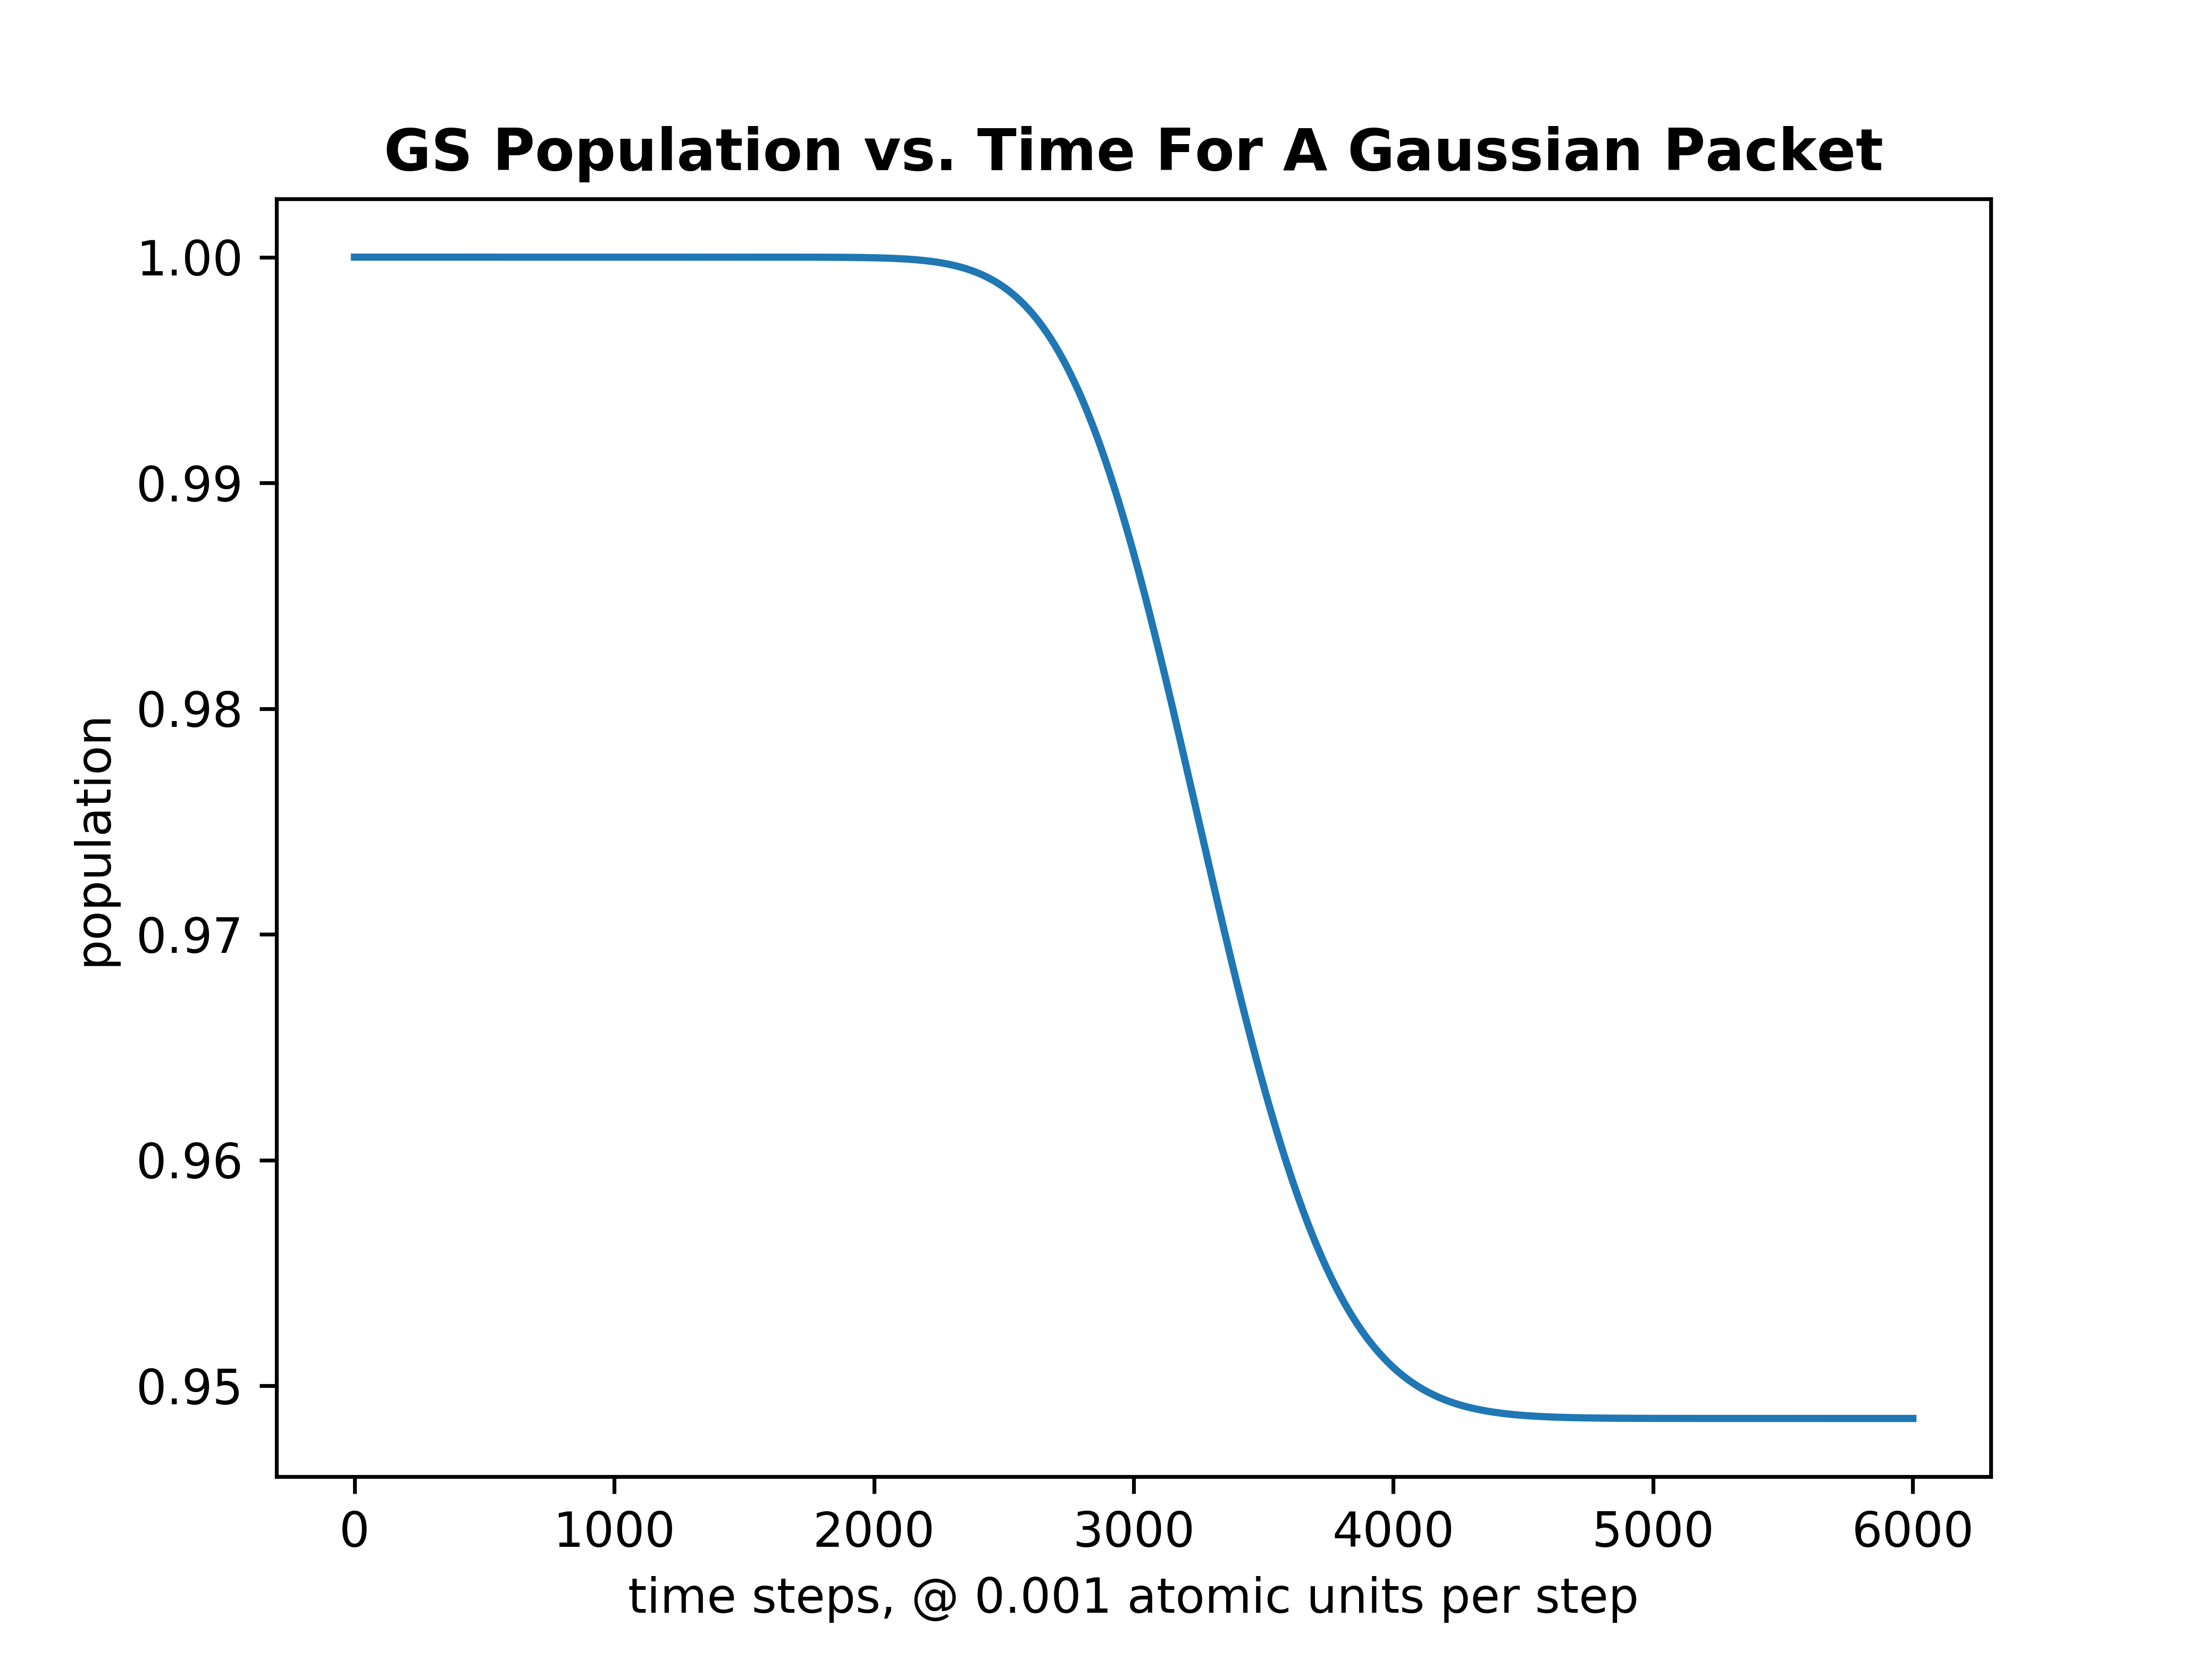
\includegraphics[width=\textwidth]{./GS1GaussianPacketNEW.png}
          \centering
          \caption{Effect of Gaussian Packet on GS population}
\end{figure}

This graph shows that between around 0.5 and 1.5 atomic units of time into the simulation, the wavefunction is rapidly excited; losing 5\% of the population by 1.5 atomic units of time. After this initial loss, the population stays steadily at around 95\% for the rest of the simulation, indicating no further change to its energy.

\section{Multiple Gaussian Packets}

We investigate the effects on our system of subjecting it to a series of gaussian potentials over the course of the simulation. 

\subsection{Potential Description}
The external potential used in this simulation is similar to the one used in the previous simulation, but with three added to the softcore potential to form the total potential term rather than one. Additionally, two of the packets have their centres shifted to occur at 3 and 5 atomic units of time.

\subsection{Effect On State Evolution}
The graphs in the figure below describe the evolution of the system as it absorbs energy from repeated gaussian potentials. This differs from the previous investigation of a single packet in that the end result is a system with noticeably higher contributions from excited states than previously, indicating that the system has absorbed more energy. Additionally, the wavefunction of the system at the end shows higher exctited state contributions than in the middle of the simulation - indicating that energy is absorbed both before and after the mid-point of the simulation, matching expectations as the packets were staggered to be centred around $\frac{1}{6}, \frac{3}{6}, \text{ and }\frac{5}{6}$ of the simulation.
\begin{figure}[H]
          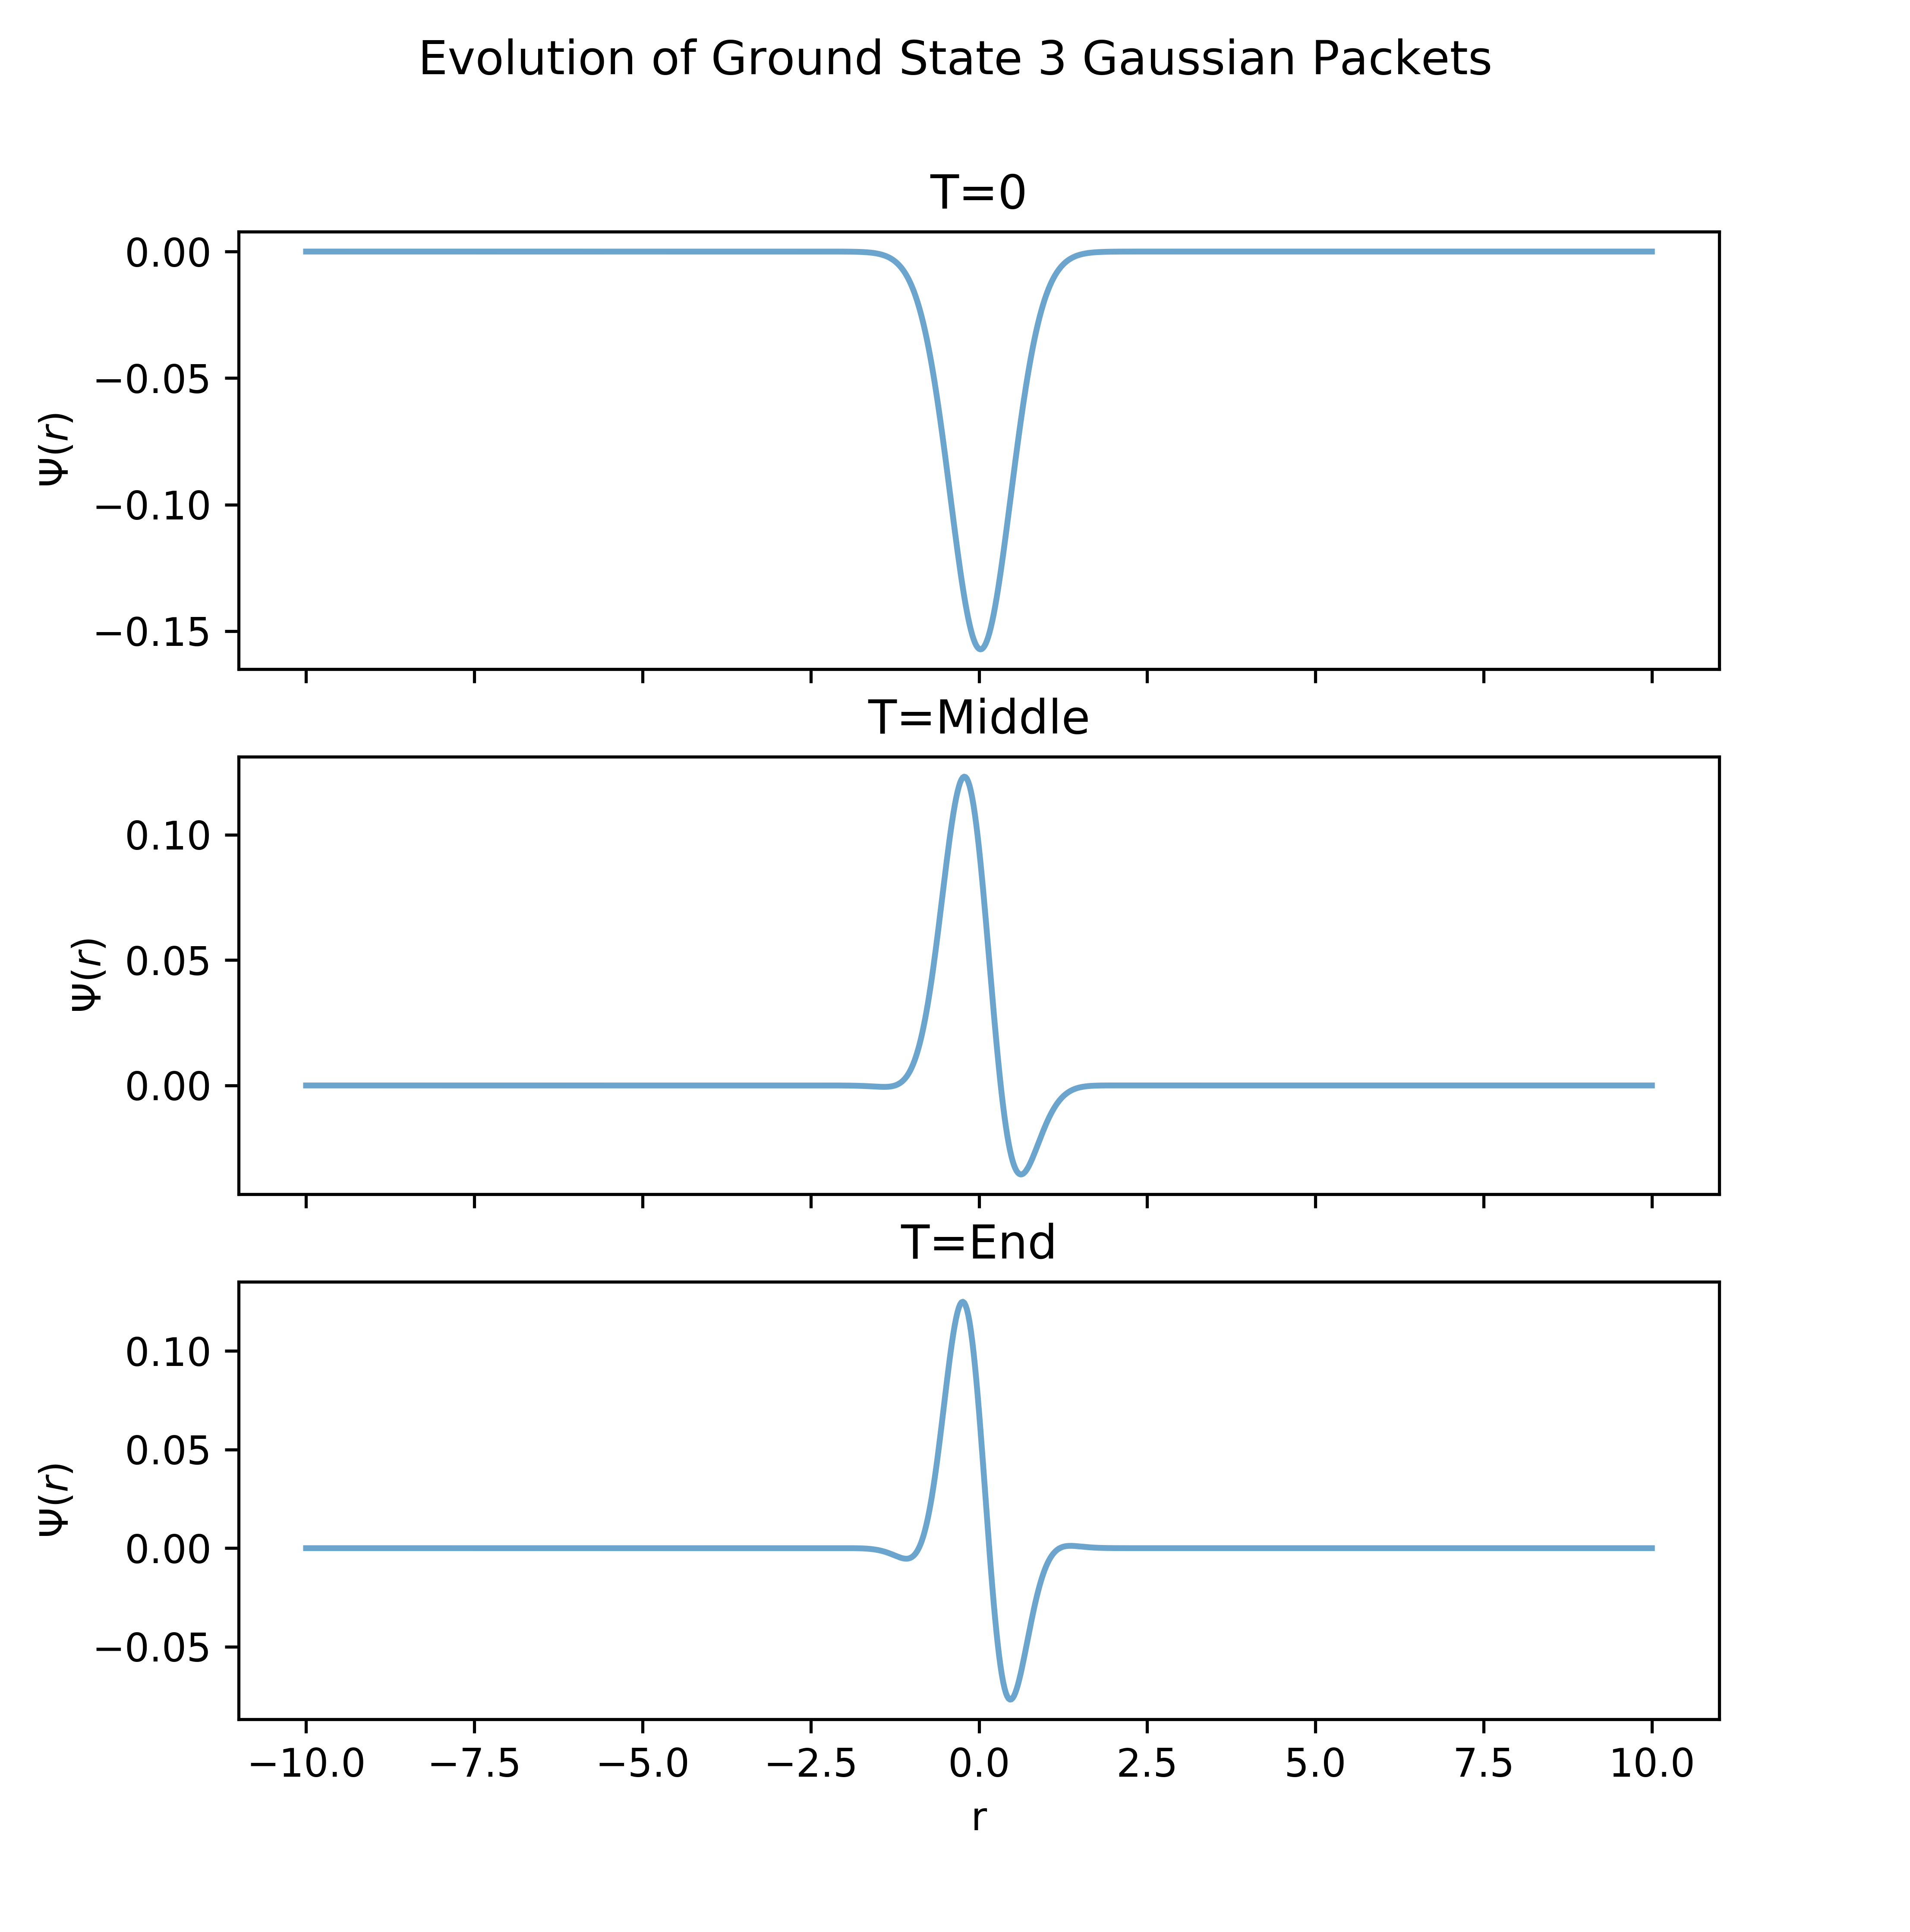
\includegraphics[width=\textwidth]{./GS3GaussianPacketNEWwavefunction.png}
          \centering
          \caption{Effect of 3 Gaussian Packets on wavefunction}
\end{figure}

The Ground State population was also investigated, with the results shown in Figure 4.6 below, and we can see that there are three distinct drops in population - centred around 1, 3, and 5 atomic units of time; matching when we placed the maxima of the packets. Additionally, we can see that the repeated gaussian packets led to a higher overall drop in Ground State population by the end of the simulation, matching the analysis of the evolution of the wavefunction where we noticed higher contributions from excited states than with the single packet.
\begin{figure}[H]
          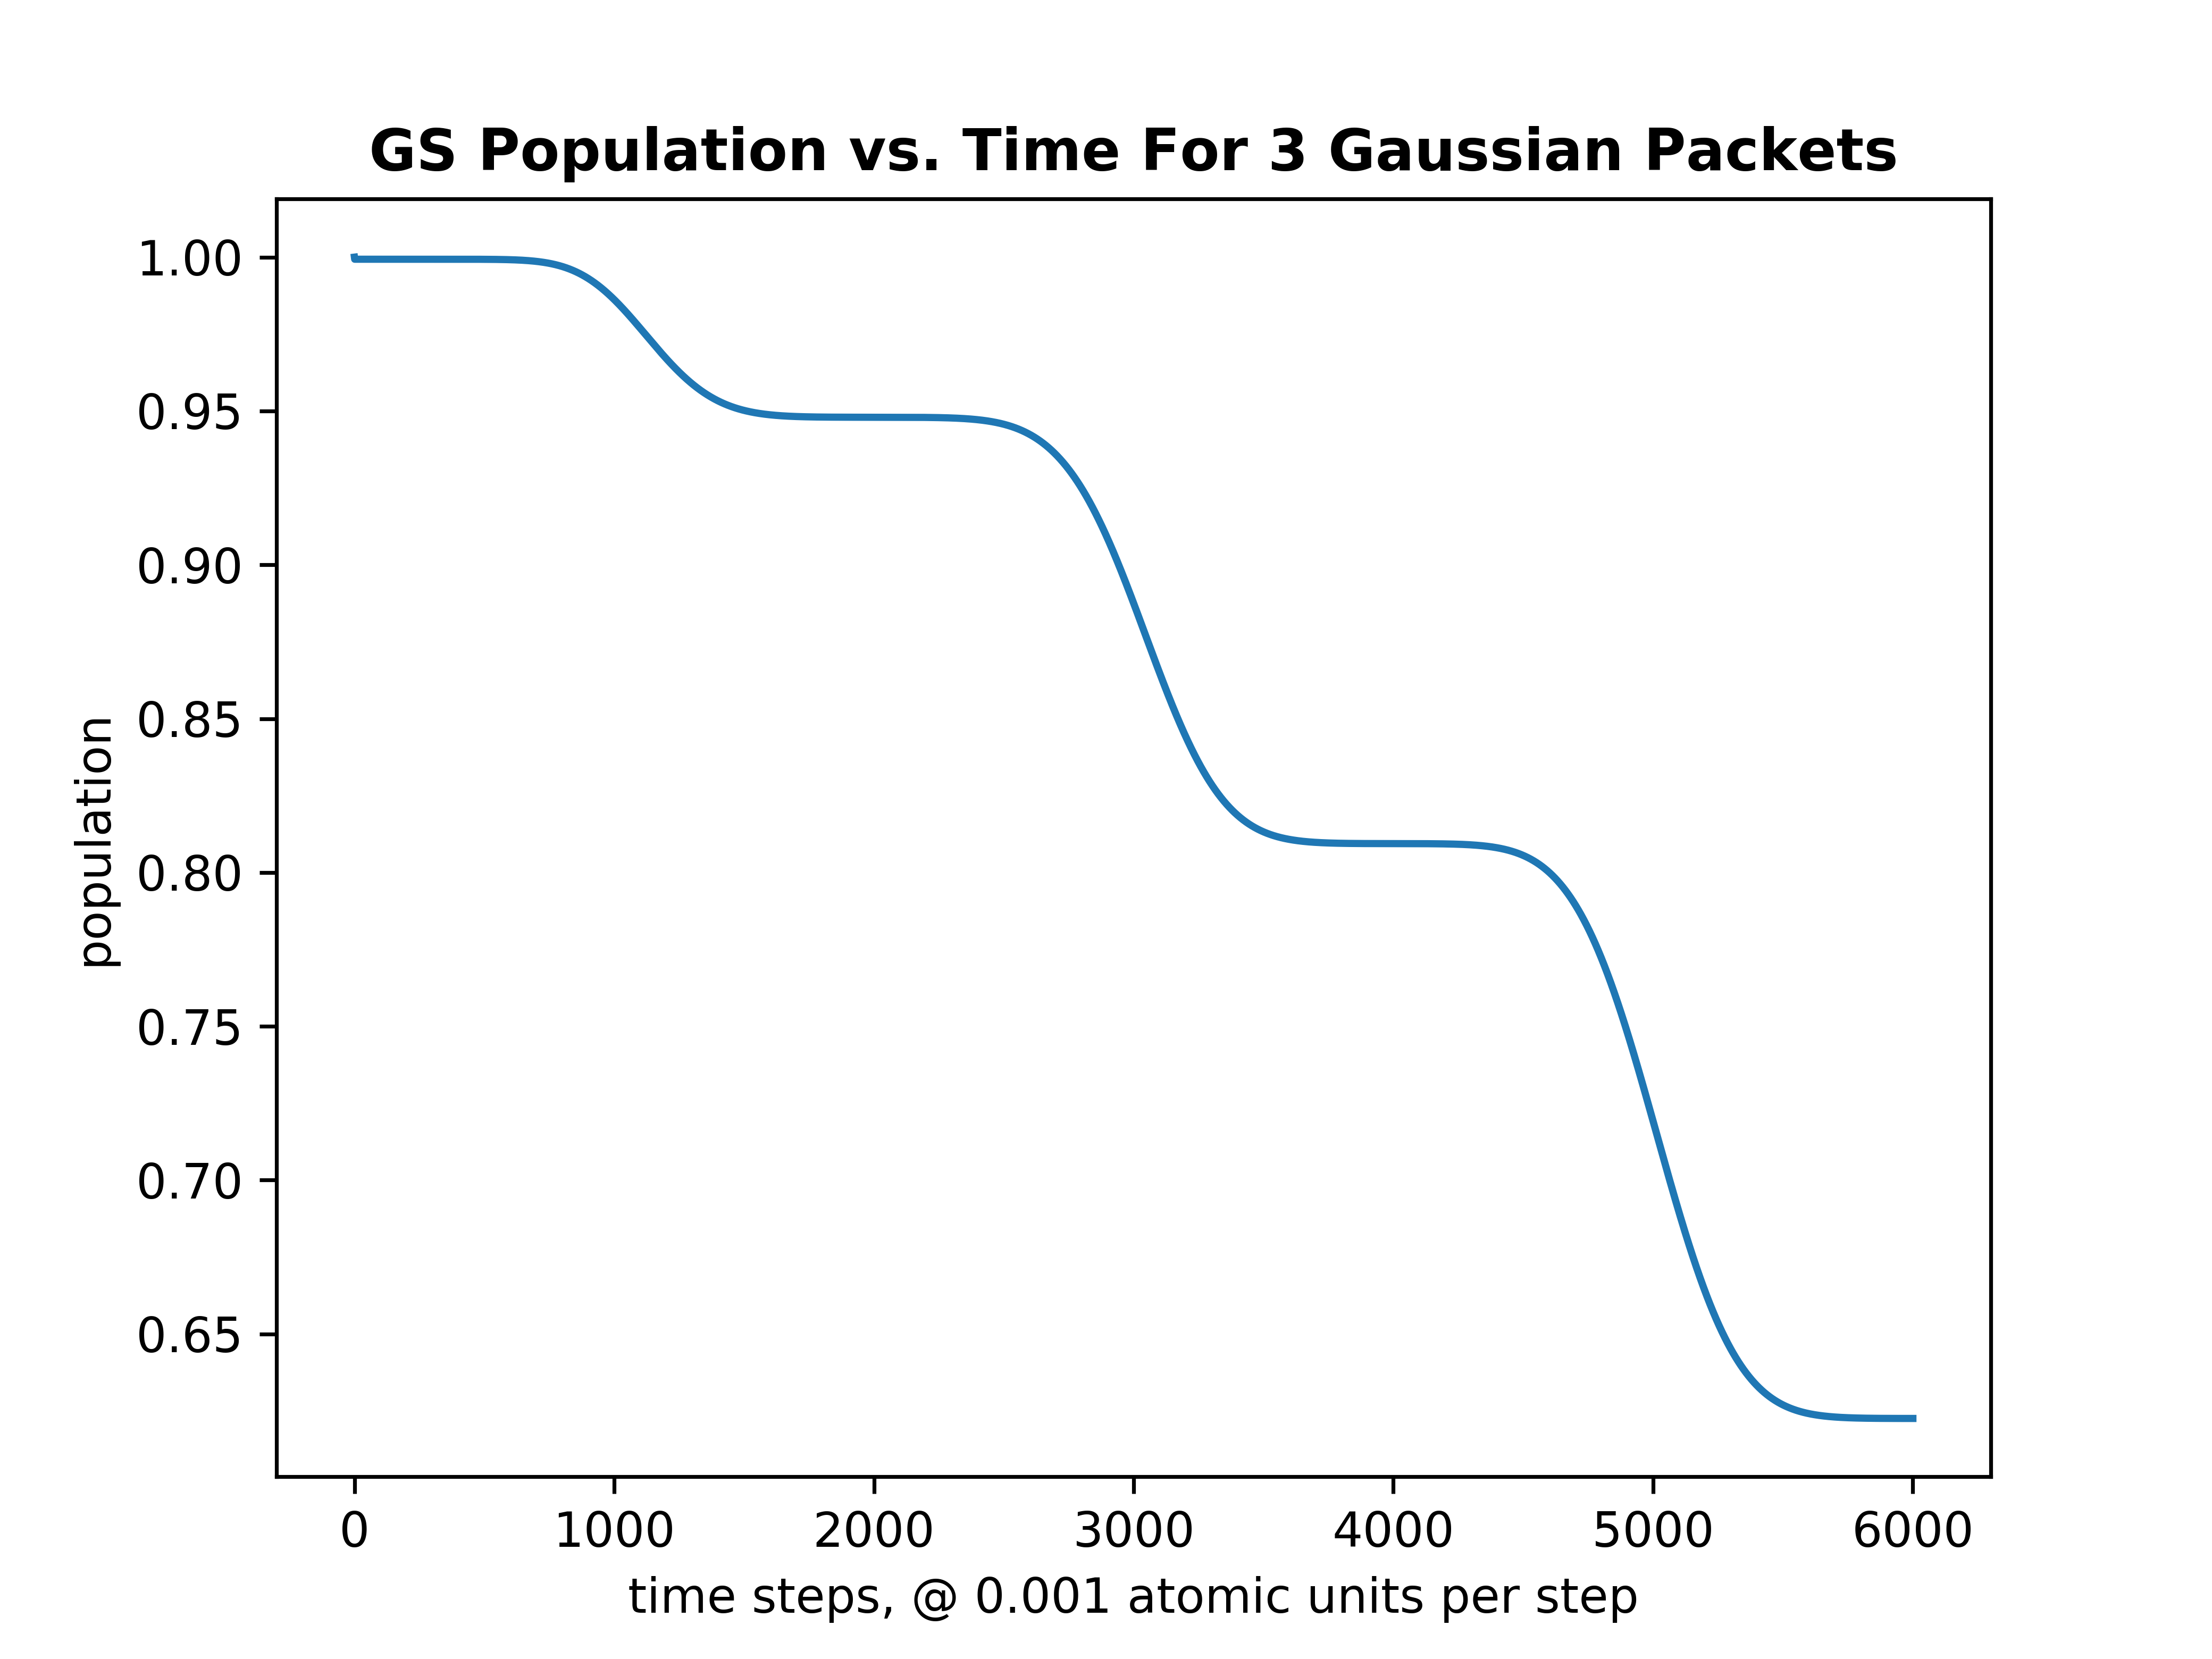
\includegraphics[width=\textwidth]{./GS3GaussianPacketNEW.png}
          \centering
          \caption{Effect of 3 Gaussian Packets on GS population}
\end{figure}

\section{Simulated Laser Pulse}

Here we model a Laser pulse interacting with our system using a potential built by encapsulating a sinusoidal wave within a gaussian packet to model our Laser pulse. Mathematically, this potential is described by;
$$
V_{\text{ext}} = \alpha \frac{2}{\sqrt{2\pi}}e^{-2\left(t-3\right)^{2}}\mathbf{r}\ \text{sin}\left(\omega t\right),
$$
where $\omega$ is the frequency of the sinusoidal term and $\alpha$ is a multiplicative factor controlling the intensity.

The figure below describes the field strength of this potential over the course of the simulation, and qualitatively demonstrates its similarity to a laser pulse potential:
\begin{figure}[H]
          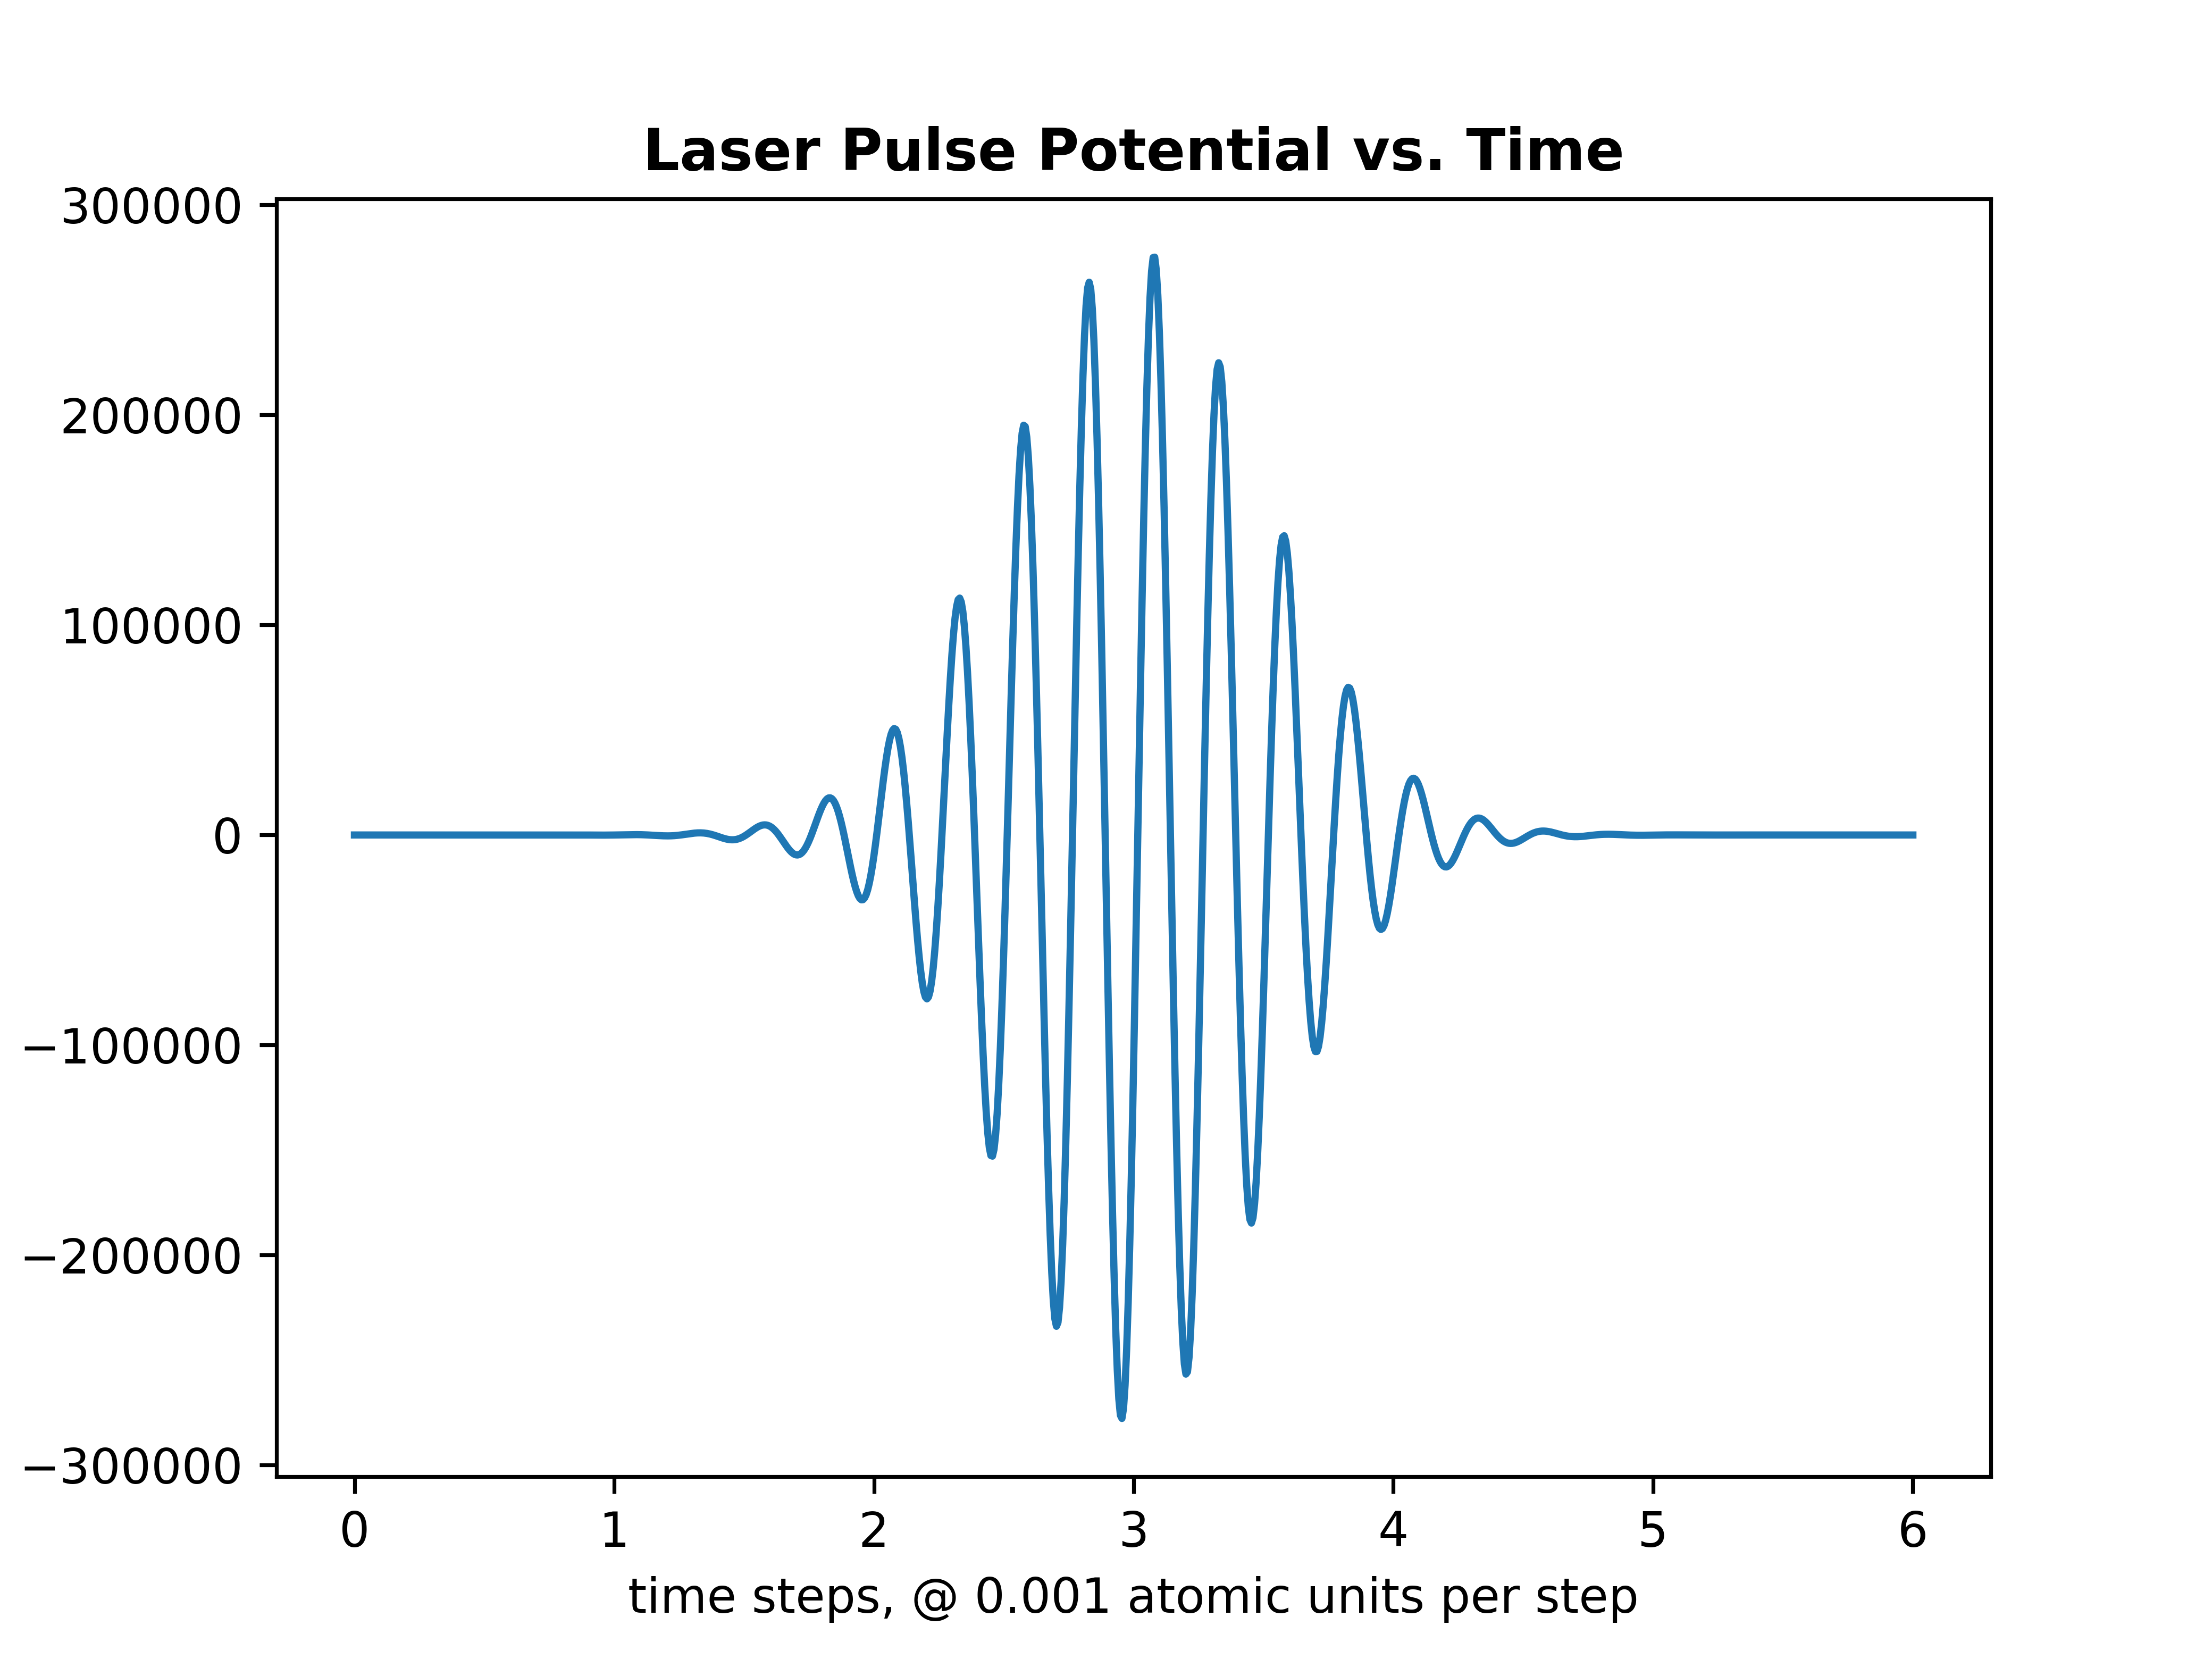
\includegraphics[width=\textwidth]{./LaserPulseNEWPotential.png}
          \centering
          \caption{Potential Field Strength Over Time For Laser Pulse}
\end{figure}

Upon interacting with our system, rapid gains and losses of energy are made as the direction of the potential cycles. The following figure demonstrates this effect;
\begin{figure}[H]
          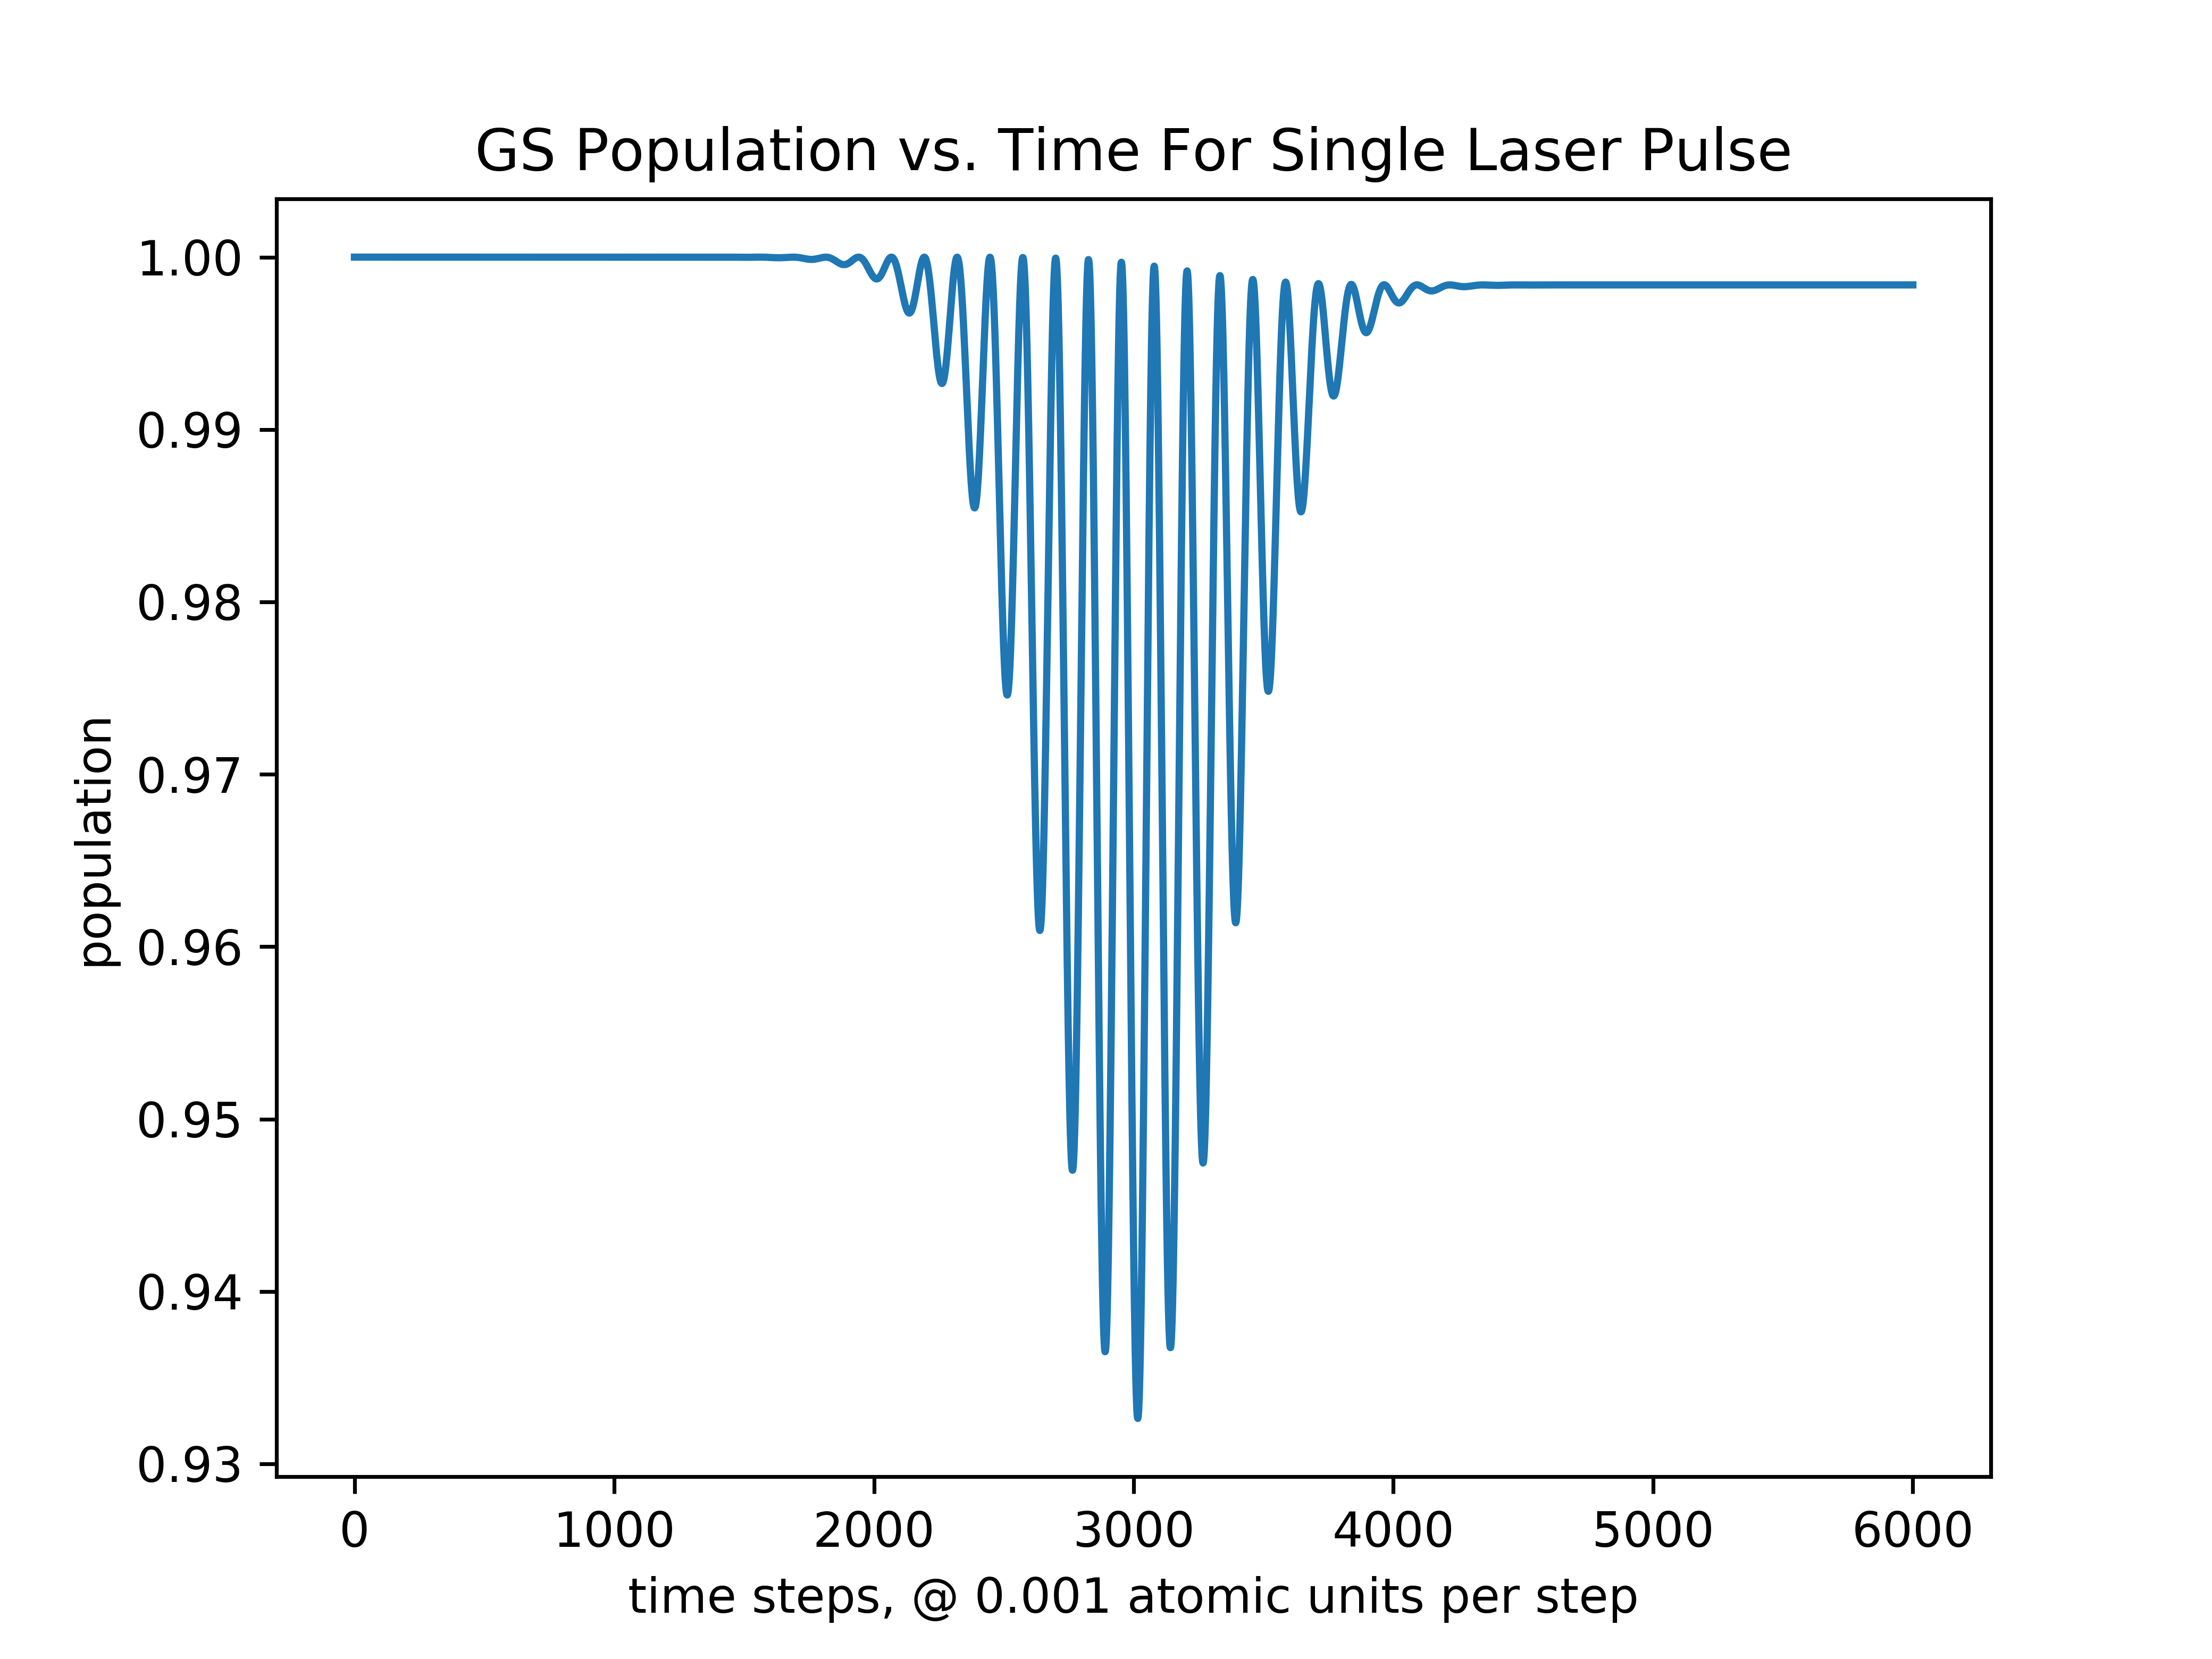
\includegraphics[width=\textwidth]{./GSSingleLaserPulseNEW.png}
          \centering
          \caption{Effect of Simulated Laser Pulse on GS population}
\end{figure}

Here we see that the wavefunction, initially entirely in the ground state, continuously gains and loses population in higher excited states as the pulse interacts - with the magnitudes of these gains and losses scaling with the magnitude of the gaussian packet enveloping the pulse. Additionally we see that almost, but not all of, the population is retained at the end of the pulse; leaving a small amount ($\simeq 1\%$) of the population in higher excited states.

%----------------------------------------------------------------------------------------
 
% Chapter 1

\chapter{RMT} % Main chapter title

\label{Chapter5} % For referencing the chapter elsewhere, use \ref{Chapter1} 

%----------------------------------------------------------------------------------------

\section{R-Matrix Theory}
\subsection{TODO 1}
df h jd nd re kfd nljd da nk kjnds 
Is this an appropriate place for the above?

\subsection{TODO 2}

The Radial TISE is a simplification of the TISE for the case where the system is spherically symmetric, which is the case for a Hydrogenic atom - for both a Coulomb Potential or a Soft-Core Potential.

\section{Overview Of Project}
\subsection{TODO 3}
lksdlkjasd kalsjdnf alksjd fakjn a lkjnasd lka a la lkjasd la lksad lak a
as akjs ka lka alk lllasd l
\subsection{TODO 4}
asdkjfnaslkdjfal lkajsnd a;kjndfajsnasdk aoa 
assdf as kjdnfasd

\section{Optimisation Of **TODO**}
\subsection{Overview Of Potential Inefficiency}
sdf gd jd kns doijsa o;noire jknf jndf 

\subsection{Method Of Attempted Improvement}
dsf lkdf lkndf lksn lkna lk
dsf gskfdn sdf 
dsf kn

\subsection{Analysis Of Effectiveness \& Usefulness Of Changes}
dsfg kjd klds lk
sd klndf lk s
sd dfg sdfgdsfgsd

\subsection{Insights}

\section{Optimisation Of **TODO**}
\subsection{Overview Of Potential Inefficiency}
sdf gd jd kns doijsa o;noire jknf jndf 

\subsection{Method Of Attempted Improvement}
dsf lkdf lkndf lksn lkna lk
dsf gskfdn sdf 
dsf kn

\subsection{Analysis Of Effectiveness \& Usefulness Of Changes}
dsfg kjd klds lk
sd klndf lk s
sd dfg sdfgdsfgsd

\subsection{Insights}

\section{Mid-Region Investigation To Improve Parallelisation}
\subsection{Communication Costs For Parallelisation In Current Inner/Outer Region Model}
sd fkjs aksn ;ksdn ;aksd sakld dsa 
sd d df 
df fds 
\subsection{Conjecture For How Addition Of Mid-Region Could Improve Speeds}
sd gfjknds lkjsdf nlkjdf nskjdf nsdkfj 

\subsection{Description Of Method Used In Attempt}
df gkl slkd flkdnf dsf
df kjdnf 

\subsection{Analysis Of Speed Improvements In Different Use Cases}
dsf jdflkm ldskfmlkfd sdflkn

\subsection{Review \& Insights Of Addition Of Mid-Region}
sd kjns dlkjnds 
skdj ns 
sdak nsd 



 

%----------------------------------------------------------------------------------------
%	THESIS CONTENT - APPENDICES
%----------------------------------------------------------------------------------------

\appendix % Cue to tell LaTeX that the following "chapters" are Appendices

% Include the appendices of the thesis as separate files from the Appendices folder
% Uncomment the lines as you write the Appendices

% Appendix A

\chapter{Frequently Asked Questions} % Main appendix title

\label{AppendixA} % For referencing this appendix elsewhere, use \ref{AppendixA}

\section{How do I change the colors of links?}

The color of links can be changed to your liking using:

{\small\verb!\hypersetup{urlcolor=red}!}, or

{\small\verb!\hypersetup{citecolor=green}!}, or

{\small\verb!\hypersetup{allcolor=blue}!}.

\noindent If you want to completely hide the links, you can use:

{\small\verb!\hypersetup{allcolors=.}!}, or even better: 

{\small\verb!\hypersetup{hidelinks}!}.

\noindent If you want to have obvious links in the PDF but not the printed text, use:

{\small\verb!\hypersetup{colorlinks=false}!}.

%\include{Appendices/AppendixB}
%\include{Appendices/AppendixC}

%----------------------------------------------------------------------------------------
%	BIBLIOGRAPHY
%----------------------------------------------------------------------------------------

\printbibliography[heading=bibintoc]

%----------------------------------------------------------------------------------------

\end{document}  
